%
\documentclass[11pt,twoside]{article}
\usepackage[letterpaper,margin=1in]{geometry}
\usepackage[utf8x]{inputenc}
\usepackage{amssymb}
\usepackage{graphicx}
\usepackage{verbatim}
\title{Generic Single Edge Fault Tolerant Exact Distance Oracle}
\author{Manoj Gupta\\
   IIT Gandhinagar, India\\
   {\small\texttt{gmanoj@iitgn.ac.in}}
 \and
Aditi Singh\\
   IIT Gandhinagar, India\\
{\small\texttt{aditi.singh@iitgn.ac.in}}
}

\usepackage{amsmath,amssymb,amsthm,xpatch}

%\setlength{\topsep}{0pt}
%\setlength{\partopsep}{0pt plus 0pt minus 0pt}
%\setlength{\parskip}{0pt}
%\setlength{\parindent}{0pt}





\usepackage{dsfont}
\usepackage{xargs}
\usepackage{todonotes}
\usepackage{tikz}
\usepackage[boxruled,lined,linesnumbered]{algorithm2e}
\usepackage{amssymb}
%\usepackage{romannum}
\usepackage{wrapfig}
%\usepackage{mathptmx}
\usepackage{mathrsfs}
\usepackage{enumerate}
\usepackage{caption}
\usepackage{microtype}
\usepackage{soul}
%\usepackage[charter]{mathdesign}
%\usepackage{hyperref}
\usepackage{enumitem}







\newtheorem{theorem}{Theorem}
\newtheorem{lemma}[theorem]{Lemma}
\newtheorem{assumption}[theorem]{Assumption}
\newtheorem{definition}[theorem]{Definition}
\newtheorem{corollary}[theorem]{Corollary}
\newtheorem{observation}[theorem]{Observation}

\newif\iflong
\longtrue

\newcommand{\TT}{\mathcal{T}}
\newcommand{\Ps}{\mathcal{P}}
\newcommand{\conc}{\diamond}
\newcommand{\DET}{\textsc{Detour}}
\newcommand{\UNQ}{\textsc{Unique}}
\newcommand{\FF}{\textsc{First}}
\newcommand{\LL}{\textsc{Last}}
\newcommand{\SBFS}{$\sigma$-\textsc{BFS}}
\newcommand{\BFS}{\textsc{BFS}}
\newcommand{\TZE}{\mathcal{R}_1}
\newcommand{\TON}{\mathcal{R}_1}
\newcommand{\TTW}{\mathcal{R}_2}
\newcommand{\RR}{\mathcal{R}}
\newcommand{\BP}{\mathcal{B}}
\newcommand{\GP}{\mathcal{G}}
\newcommand{\INT}{\textsc{Int}}
\newcommand{\BST}{\textsc{Bst}}
\newcommand{\RMQ}{\textsc{Rmq}}
\newcommand{\HE}{\textsc{Heavy}}
\newcommand{\LI}{\textsc{Light}}
\newcommand{\QQ}{\textsc{Q}}

%\setlength{\textwidth}{6.5in}
%\setlength{\oddsidemargin}{0.0in}
%\setlength{\textheight}{9.2in}
%\addtolength{\topmargin}{-.875in}



\begin{document}



\maketitle

  In this paper, we explore the connection between secret key agreement and secure omniscience within the setting of the multiterminal source model with a wiretapper who has side information. While the secret key agreement problem considers the generation of a maximum-rate secret key through public discussion, the secure omniscience problem is concerned with communication protocols for omniscience that minimize the rate of information leakage to the wiretapper. The starting point of our work is a lower bound on the minimum leakage rate for omniscience, $\rl$, in terms of the wiretap secret key capacity, $\wskc$. Our interest is in identifying broad classes of sources for which this lower bound is met with equality, in which case we say that there is a duality between secure omniscience and secret key agreement. We show that this duality holds in the case of certain finite linear source (FLS) models, such as two-terminal FLS models and pairwise independent network models on trees with a linear wiretapper. Duality also holds for any FLS model in which $\wskc$ is achieved by a perfect linear secret key agreement scheme. We conjecture that the duality in fact holds unconditionally for any FLS model. On the negative side, we give an example of a (non-FLS) source model for which duality does not hold if we limit ourselves to communication-for-omniscience protocols with at most two (interactive) communications.  We also address the secure function computation problem and explore the connection between the minimum leakage rate for computing a function and the wiretap secret key capacity.
  
%   Finally, we demonstrate the usefulness of our lower bound on $\rl$ by using it to derive equivalent conditions for the positivity of $\wskc$ in the multiterminal model. This extends a recent result of Gohari, G\"{u}nl\"{u} and Kramer (2020) obtained for the two-user setting.
  
   
%   In this paper, we study the problem of secret key generation through an omniscience achieving communication that minimizes the 
%   leakage rate to a wiretapper who has side information in the setting of multiterminal source model.  We explore this problem by deriving a lower bound on the wiretap secret key capacity $\wskc$ in terms of the minimum leakage rate for omniscience, $\rl$. 
%   %The former quantity is defined to be the maximum secret key rate achievable, and the latter one is defined as the minimum possible leakage rate about the source through an omniscience scheme to a wiretapper. 
%   The main focus of our work is the characterization of the sources for which the lower bound holds with equality \textemdash it is referred to as a duality between secure omniscience and wiretap secret key agreement. For general source models, we show that duality need not hold if we limit to the communication protocols with at most two (interactive) communications. In the case when there is no restriction on the number of communications, whether the duality holds or not is still unknown. However, we resolve this question affirmatively for two-user finite linear sources (FLS) and pairwise independent networks (PIN) defined on trees, a subclass of FLS. Moreover, for these sources, we give a single-letter expression for $\wskc$. Furthermore, in the direction of proving the conjecture that duality holds for all FLS, we show that if $\wskc$ is achieved by a \emph{perfect} secret key agreement scheme for FLS then the duality must hold. All these results mount up the evidence in favor of the conjecture on FLS. Moreover, we demonstrate the usefulness of our lower bound on $\wskc$ in terms of $\rl$ by deriving some equivalent conditions on the positivity of secret key capacity for multiterminal source model. Our result indeed extends the work of Gohari, G\"{u}nl\"{u} and Kramer in two-user case.
\newpage
% !TEX root = ../arxiv.tex

Unsupervised domain adaptation (UDA) is a variant of semi-supervised learning \cite{blum1998combining}, where the available unlabelled data comes from a different distribution than the annotated dataset \cite{Ben-DavidBCP06}.
A case in point is to exploit synthetic data, where annotation is more accessible compared to the costly labelling of real-world images \cite{RichterVRK16,RosSMVL16}.
Along with some success in addressing UDA for semantic segmentation \cite{TsaiHSS0C18,VuJBCP19,0001S20,ZouYKW18}, the developed methods are growing increasingly sophisticated and often combine style transfer networks, adversarial training or network ensembles \cite{KimB20a,LiYV19,TsaiSSC19,Yang_2020_ECCV}.
This increase in model complexity impedes reproducibility, potentially slowing further progress.

In this work, we propose a UDA framework reaching state-of-the-art segmentation accuracy (measured by the Intersection-over-Union, IoU) without incurring substantial training efforts.
Toward this goal, we adopt a simple semi-supervised approach, \emph{self-training} \cite{ChenWB11,lee2013pseudo,ZouYKW18}, used in recent works only in conjunction with adversarial training or network ensembles \cite{ChoiKK19,KimB20a,Mei_2020_ECCV,Wang_2020_ECCV,0001S20,Zheng_2020_IJCV,ZhengY20}.
By contrast, we use self-training \emph{standalone}.
Compared to previous self-training methods \cite{ChenLCCCZAS20,Li_2020_ECCV,subhani2020learning,ZouYKW18,ZouYLKW19}, our approach also sidesteps the inconvenience of multiple training rounds, as they often require expert intervention between consecutive rounds.
We train our model using co-evolving pseudo labels end-to-end without such need.

\begin{figure}[t]%
    \centering
    \def\svgwidth{\linewidth}
    \input{figures/preview/bars.pdf_tex}
    \caption{\textbf{Results preview.} Unlike much recent work that combines multiple training paradigms, such as adversarial training and style transfer, our approach retains the modest single-round training complexity of self-training, yet improves the state of the art for adapting semantic segmentation by a significant margin.}
    \label{fig:preview}
\end{figure}

Our method leverages the ubiquitous \emph{data augmentation} techniques from fully supervised learning \cite{deeplabv3plus2018,ZhaoSQWJ17}: photometric jitter, flipping and multi-scale cropping.
We enforce \emph{consistency} of the semantic maps produced by the model across these image perturbations.
The following assumption formalises the key premise:

\myparagraph{Assumption 1.}
Let $f: \mathcal{I} \rightarrow \mathcal{M}$ represent a pixelwise mapping from images $\mathcal{I}$ to semantic output $\mathcal{M}$.
Denote $\rho_{\bm{\epsilon}}: \mathcal{I} \rightarrow \mathcal{I}$ a photometric image transform and, similarly, $\tau_{\bm{\epsilon}'}: \mathcal{I} \rightarrow \mathcal{I}$ a spatial similarity transformation, where $\bm{\epsilon},\bm{\epsilon}'\sim p(\cdot)$ are control variables following some pre-defined density (\eg, $p \equiv \mathcal{N}(0, 1)$).
Then, for any image $I \in \mathcal{I}$, $f$ is \emph{invariant} under $\rho_{\bm{\epsilon}}$ and \emph{equivariant} under $\tau_{\bm{\epsilon}'}$, \ie~$f(\rho_{\bm{\epsilon}}(I)) = f(I)$ and $f(\tau_{\bm{\epsilon}'}(I)) = \tau_{\bm{\epsilon}'}(f(I))$.

\smallskip
\noindent Next, we introduce a training framework using a \emph{momentum network} -- a slowly advancing copy of the original model.
The momentum network provides stable, yet recent targets for model updates, as opposed to the fixed supervision in model distillation \cite{Chen0G18,Zheng_2020_IJCV,ZhengY20}.
We also re-visit the problem of long-tail recognition in the context of generating pseudo labels for self-supervision.
In particular, we maintain an \emph{exponentially moving class prior} used to discount the confidence thresholds for those classes with few samples and increase their relative contribution to the training loss.
Our framework is simple to train, adds moderate computational overhead compared to a fully supervised setup, yet sets a new state of the art on established benchmarks (\cf \cref{fig:preview}).

\section{Preliminaries}
Given a graph $G=(V,E)$, and vertex $u \in V$, let $\deg(u,G)$ be the degree of $u$ in $G$. 
Given a tree $T$ and $u, v \in T$, denote the $u$-$v$ path in $T$ by $\pi(u,v,T)$. When the tree $T$ is clear from the context, we may omit it and write $\pi(u,v)$. For a (possibly weighted) subgraph $G' \subseteq G$ and a vertex pair $s,t \in V$, let $\dist_{G'}(s,t)$ denote the length of the $s$-$t$ shortest path in $G'$. 

\paragraph{Fault-Tolerant Labeling Schemes.}
For a given graph $G$, let $\Pi: V\times V \times \mathcal{G} \to \mathbb{R}_{\geq 0}$ %\mtodo{a reviewer pointed out that the last element in the domain should probably be subgraphs of $G$ and not $G$, see which notation we want here.} \mertodo{I am not sure that it is needed as we consider $G$ in the fault-free setting and $G \setminus F$ in the FT setting. We can of course write $\Pi: V\times V \times \mathcal{G} \to \mathbb{R}_{\geq 0}$ where $\mathcal{G}$ is the family of all $G$-subgraphs, but I cannot see why we need it.} 
be a function defined on pairs of vertices and a subgraph $G' \subset G$, where $\mathcal{G}$ is the family of all subgraphs of $G$. For an integer parameter $f\geq 1$, an $f$-\emph{fault-tolerant labeling scheme} for a function $\Pi$ and a graph family $\mathcal{F}$ is a pair of functions $(L_{\Pi},D_{\Pi})$. The function $L_{\Pi}$ is called the \emph{labeling function}, and $D_{\Pi}$ is called the \emph{decoding function}. For every graph $G$ in the family $\mathcal{F}$, the labeling function $L_{\Pi}$ associates with each vertex $u \in V(G)$ and every edge $e \in E(G)$, a label $L_{\Pi}(u,G)$ (resp., $L_{\Pi}(e,G)$). It is then required that given the labels of any triplets $s,t, F \in V \times V \times E^f$, the decoding function $D_{\Pi}$ computes $\Pi(s,t, G \setminus F)$.  The primary complexity measure of a labeling scheme is the \emph{label length}, measured by the length (in bits) of the largest label it assigns to some vertices (or edges) in $G$ over all graphs $G \in \mathcal{F}$. An $f$-FT connectivity labeling scheme is required to output YES iff $s$ and $t$ are connected in $G \setminus F$.  In $f$-FT \emph{approximate distance labeling scheme} it is required to output an estimate for the $s$-$t$ distance in the graph $G \setminus F$. Formally, an $f$-FT labeling scheme is $q$\emph{-approximate} if the value $\delta(s,t,F)$ returned by the decoder algorithm satisfies that $\dist_{G \setminus F}(s,t)\leq \delta(s,t,F) \leq q \cdot \dist_{G \setminus F}(s,t)$.  Throughout the paper we provide randomized labeling schemes which provide a high probability guarantee of correctness for any fixed triplet $\langle s,t, F \rangle$. 


\paragraph{Fault-Tolerant Routing Schemes.} In the setting of FT routing scheme, one is given a pair of source $s$ and destination $t$ as well as $F$ edge faults, which are initially unknown to $s$. The routing scheme consists of \emph{preprocessing} and \emph{routing} algorithms. The preprocessing algorithm defines labels $L(u)$ to each of the vertices $u$, and a header $H(M)$ to the designated message $M$. In addition, it defines for every vertex $u$ a routing table $R(u)$. The labels and headers are usually required to be short, i.e., of poly-logarithmic bits. 
The routing procedure determines at each vertex $u$ the port-number on which $u$ should send the messages it receives. The computation of the next-hop is done by considering the header of the message $H(M)$, the label of the source and destination $L(s)$ and $L(t)$ and the routing table $R(u)$. The routing procedure at vertex $u$ might also edit the header of the message $H(M)$. The failing edges are not known in advance and can only be revealed by reaching (throughout the message routing) one of their endpoints. The \emph{space} of the scheme is determined based on maximal length of message headers, labels and the individual routing tables. The stretch of the scheme is measured by the ratio between the length of the path traversed until the message arrived its destination and the length of the shortest $s$-$t$ path in $G \setminus F$. In the more relaxed setting of \emph{forbidden-set routing schemes} the failing edges are given as input to the routing algorithm.

%\paragraph{Forbidden-Set Routing Schemes.} One of the key applications of labeling schemes is routing.
%In the setting of forbidden-set routing schemes, given the labels of $s$, $t$ and a set of forbidden edges $
%F$, it is required to determine the next-hop neighbor of $s$ on some short $s$-$t$ path in $G \setminus F$. The main two complexity measures are the stretch induced by the $s$-$t$ path encoded by the labels.  \mtodo{Maybe the definition should be more similar to the next one? (consider labels, tables, headers)}
%That is, given the labels of $u$, $v$ and the faults $F$, the decoder function returns the port-number of $u$'s neighbor lying on a $u$-$v$ path $P$ in $G \setminus F$ such that $P \subseteq G$ and $len(P)\leq s \cdot \dist(u,v, G \setminus F)$ for some approximation factor $s$. 

\section{Our Approach}
We formulate the problem as an anisotropic diffusion process and the diffusion tensor is learned through a deep CNN directly from the given image, which guides the refinement of the output.

\begin{figure}[t]
\includegraphics[width=1.0\textwidth]{fig/CSPN_SPN2.pdf}
\caption{Comparison between the propagation process in SPN~\cite{liu2017learning} and CPSN in this work.}
\label{fig:compare}
\end{figure}

\subsection{Convolutional Spatial Propagation Network}
% demonstrate the thereom is hold when turns to be convolution.
Given a depth map $D_o \in \spa{R}^{m\times n}$ that is output from a network, and image $\ve{X} \in \spa{R}^{m\times n}$, our task is to update the depth map to a new depth map $D_n$ within $N$ iteration steps, which first reveals more details of the image, and second improves the per-pixel depth estimation results. 

\figref{fig:compare}(b) illustrates our updating operation. Formally, without loss of generality, we can embed the $D_o$ to some hidden space $\ve{H} \in \spa{R}^{m \times n \times c}$. The convolutional transformation functional with a kernel size of $k$ for each time step $t$ could be written as,
\begin{align}
    \ve{H}_{i, j, t + 1} &= \sum\nolimits_{a,b = -(k-1)/2}^{(k-1)/2} \kappa_{i,j}(a, b) \odot \ve{H}_{i-a, j-b, t} \nonumber \\
\mbox{where,~~~~}
    \kappa_{i,j}(a, b) &= \frac{\hat{\kappa}_{i,j}(a, b)}{\sum_{a,b, a, b \neq 0} |\hat{\kappa}_{i,j}(a, b)|}, \nonumber\\
    \kappa_{i,j}(0, 0) &= 1 - \sum\nolimits_{a,b, a, b \neq 0}\kappa_{i,j}(a, b)
\label{eqn:cspn}
\end{align}
where the transformation kernel $\hat{\kappa}_{i,j} \in \spa{R}^{k\times k \times c}$ is the output from an affinity network, which is spatially dependent on the input image. The kernel size $k$ is usually set as an odd number so that the computational context surrounding pixel $(i, j)$ is symmetric.
$\odot$ is element-wise product. Following~\cite{liu2017learning}, we normalize kernel weights between range of $(-1, 1)$ so that the model can be stabilized and converged by satisfying the condition $\sum_{a,b, a,b \neq 0} |\kappa_{i,j}(a, b)| \leq 1$. Finally, we perform this iteration $N$ steps to reach a stationary distribution.

% theorem, it follows diffusion with PDE 
%\addlinespace
\noindent\textbf{Correspondence to diffusion process with a partial differential equation (PDE).} \\
Similar with~\cite{liu2017learning}, here we show that our CSPN holds all the desired properties of SPN.
Formally, we can rewrite the propagation in \equref{eqn:cspn} as a process of diffusion evolution by first doing column-first vectorization of feature map $\ve{H}$ to $\ve{H}_v \in \spa{R}^{\by{mn}{c}}$.
\begin{align}
     \ve{H}_v^{t+1} = 
     \begin{bmatrix}
    1-\lambda_{0, 0}  & \kappa_{0,0}(1,0) & \cdots & 0 \\
    \kappa_{1,0}(-1,0)   & 1-\lambda_{1, 0} & \cdots & 0 \\
    \vdots & \vdots & \ddots & \vdots \\
    \vdots & \cdots & \cdots & 1-\lambda_{m,n} \\
\end{bmatrix} = \ve{G}\ve{H}_v^{t}
\label{eqn:vector}
\end{align}
where $\lambda_{i, j} = \sum_{a,b}\kappa_{i,j}(a,b)$ and $\ve{G}$ is a $\by{mn}{mn}$ transformation matrix. The diffusion process expressed with a partial differential equation (PDE) is derived as follows, 
\begin{align}
     \ve{H}_v^{t+1} &= \ve{G}\ve{H}_v^{t} = (\ve{I} - \ve{D} + \ve{A})\ve{H}_v^{t} \nonumber\\
     \ve{H}_v^{t+1} - \ve{H}_v^{t} &= - (\ve{D} - \ve{A}) \ve{H}_v^{t} \nonumber\\
     \partial_t \ve{H}_v^{t+1} &= -\ve{L}\ve{H}_v^{t}
\label{eqn:proof}
\end{align}
where $\ve{L}$ is the Laplacian matrix, $\ve{D}$ is the diagonal matrix containing all the $\lambda_{i, j}$, and $\ve{A}$ is the affinity matrix which is the off diagonal part of $\ve{G}$.

In our formulation, different from~\cite{liu2017learning} which scans the whole image in four directions~(\figref{fig:compare}(a)) sequentially, CSPN propagates a local area towards all directions at each step~(\figref{fig:compare}(b)) simultaneously, \ie with~\by{k}{k} local context, while larger context is observed when recurrent processing is performed, and the context acquiring rate is in an order of $O(kN)$.

In practical, we choose to use convolutional operation due to that it can be efficiently implemented through image vectorization, yielding real-time performance in depth refinement tasks.

Principally, CSPN could also be derived from loopy belief propagation with sum-product algorithm~\cite{kschischang2001factor}. However, since our approach adopts linear propagation, which is efficient while just a special case of pairwise potential with L2 reconstruction loss in graphical models. Therefore, to make it more accurate, we call our strategy convolutional spatial propagation in the field of diffusion process.

\begin{figure}[t]
\centering
\includegraphics[width=0.9\textwidth]{fig/hist.pdf}
\caption {(a) Histogram of RMSE with depth maps from~\cite{Ma2017SparseToDense} at given sparse depth points.  (b) Comparison of gradient error between depth maps with sparse depth replacement (blue bars) and with ours CSPN (green bars), where ours is much smaller. Check~\figref{fig:gradient} for an example. Vertical axis shows the count of pixels.}
\label{fig:hist}
\end{figure}

\subsection{Spatial Propagation with Sparse Depth Samples}
In this application, we have an additional sparse depth map $D_s$ (\figref{fig:gradient}(b)) to help estimate a depth depth map from a RGB image. Specifically, a sparse set of pixels are set with real depth values from some depth sensors, which can be used to guide our propagation process. 

Similarly, we also embed the sparse depth map $D_s = \{d_{i,j}^s\}$ to a hidden representation $\ve{H}^s$,  and we can write the updating equation of $\ve{H}$ by simply adding a replacement step after performing \equref{eqn:cspn}, 
\begin{align}
    \ve{H}_{i, j, t+1} = (1 - m_{i, j}) \ve{H}_{i, j, t+1}  +  m_{i, j} \ve{H}_{i, j}^s 
\label{eqn:cspn_sp}
\end{align}
where $m_{i, j} = \spa{I}(d_{i, j}^s > 0)$ is an indicator for the availability of sparse depth at $(i, j)$. 

In this way, we guarantee that our refined depths have the exact same value at those valid pixels in sparse depth map. Additionally, we propagate the information from those sparse depth to its surrounding pixels such that the smoothness between the sparse depths and their neighbors are maintained. 
Thirdly, thanks to the diffusion process, the final depth map is well aligned with image structures. 
This fully satisfies the desired three properties for this task which is discussed in our introduction (\ref{sec:intro}). 

% it performs a non-symmetric propagation where the information can only be diffused from the given sparse depth to others, while not the other way around.

% still follows PDE
In addition, this process is still following the diffusion process with PDE, where the transformation matrix can be built by simply replacing the rows satisfying $m_{i, j} = 1$ in $\ve{G}$ (\equref{eqn:vector}), which are corresponding to sparse depth samples, by $\ve{e}_{i + j*m}^T$. Here $\ve{e}_{i + j*m}$ is an unit vector with the value at $i + j*m$ as 1.
Therefore, the summation of each row is still $1$, and obviously the stabilization still holds in this case.

\begin{figure}[t]
\centering
\includegraphics[width=0.95\textwidth]{fig/fig2.pdf}
\caption{Comparison of depth map~\cite{Ma2017SparseToDense} with sparse depth replacement and with our CSPN \wrt smoothness of depth gradient at sparse depth points. (a) Input image. (b) Sparse depth points. (c) Depth map with sparse depth replacement. (d) Depth map with our CSPN with sparse depth points. We highlight the differences in the red box.}
\label{fig:gradient}
\end{figure}

Our strategy has several advantages over the previous state-of-the-art sparse-to-dense methods~\cite{Ma2017SparseToDense,LiaoHWKYL16}.
In \figref{fig:hist}(a), we plot a histogram of depth displacement from ground truth at given sparse depth pixels from the output of Ma \etal~\cite{Ma2017SparseToDense}. It shows the accuracy of sparse depth points cannot preserved, and some pixels could have very large displacement (0.2m), indicating that directly training a CNN for depth prediction does not preserve the value of real sparse depths provided. To acquire such property, 
one may simply replace the depths from the outputs with provided sparse depths at those pixels, however, it yields non-smooth depth gradient \wrt surrounding pixels. 
In~\figref{fig:gradient}(c), we plot such an example, at right of the figure, we compute Sobel gradient~\cite{sobel2014history} of the depth map along x direction, where we can clearly see that the gradients surrounding pixels with replaced depth values are non-smooth.
We statistically verify this in \figref{fig:hist}(b) using 500 sparse samples, the blue bars are the histogram of gradient error  at sparse pixels by comparing the gradient of the depth map with sparse depth replacement and of ground truth depth map. We can see the difference is significant, 2/3 of the sparse pixels has large gradient error.
Our method, on the other hand, as shown with the green bars in \figref{fig:hist}(b), the average gradient error is much smaller, and most pixels have zero error. In\figref{fig:gradient}(d), we show the depth gradients surrounding sparse pixels are smooth and close to ground truth, demonstrating the effectiveness of our propagation scheme. 

% Finally, in our experiments~\ref{sec:exp}, we validate the number of iterations $N$ and kernel size $k$ used for doing the CSPN.


\subsection{Complexity Analysis}
\label{subsec:time}

As formulated in~\equref{eqn:cspn}, our CSPN takes the operation of convolution, where the complexity of using CUDA with GPU for one step CSPN is $O(\log_2(k^2))$, where $k$ is the kernel size. This is because CUDA uses parallel sum reduction, which has logarithmic complexity. In addition,  convolution operation can be performed parallel for all pixels and channels, which has a constant complexity of $O(1)$. Therefore, performing $N$-step propagation, the overall complexity for CSPN is $O(\log_2(k^2)N)$, which is irrelevant to image size $(m, n)$.

SPN~\cite{liu2017learning} adopts scanning row/column-wise propagation in four directions. Using $k$-way connection and running in parallel, the complexity for one step is $O(\log_2(k))$. The propagation needs to scan full image from one side to another, thus the complexity for SPN is $O(\log_2(k)(m + n))$. Though this is already more efficient than the densely connected CRF proposed by~\cite{philipp2012dense}, whose implementation complexity with permutohedral lattice is $O(mnN)$, ours $O(\log_2(k^2)N)$ is more efficient since the number of iterations $N$ is always much smaller than the size of image $m, n$. We show in our experiments (\secref{sec:exp}), with $k=3$ and $N=12$, CSPN already outperforms SPN with a large margin (relative $30\%$), demonstrating both efficiency and effectiveness of the proposed approach.


\subsection{End-to-End Architecture}
\label{subsec:unet}
\begin{figure}[t]
\centering
\includegraphics[width=0.95\textwidth,height=0.45\textwidth]{fig/framework2.pdf}
\caption{Architecture of our networks with mirror connections for  depth estimation via transformation kernel prediction with CSPN (best view in color). Sparse depth is an optional input, which can be embedded into the CSPN to guide the depth refinement.}
\label{fig:arch}
\end{figure}

We now explain our end-to-end network architecture to predict both the transformation kernel and the depth value, which are the inputs to CSPN for depth refinement.
 As shown in \figref{fig:arch}, our network has some similarity with that from Ma \etal~\cite{Ma2017SparseToDense}, with the final CSPN layer that outputs a dense depth map.  
 
For predicting the transformation kernel $\kappa$ in \equref{eqn:cspn}, 
rather than building a new deep network for learning affinity same as Liu \etal~\cite{liu2017learning}, we branch an additional output from the given network, which shares the same feature extractor with the depth network. This helps us to save memory and time cost for joint learning of both depth estimation and transformation kernels prediction. 

Learning of affinity is dependent on fine grained spatial details of the input image. However, spatial information is weaken or lost with the down sampling operation during the forward process of the ResNet in~\cite{laina2016deeper}. Thus, we add mirror connections similar with the U-shape network~\cite{ronneberger2015u} by directed concatenating the feature from encoder to up-projection layers as illustrated by ``UpProj$\_$Cat'' layer in~\figref{fig:arch}. Notice that it is important to carefully select the end-point of mirror connections. Through experimenting three possible positions to append the connection, \ie after \textit{conv}, after \textit{bn} and after \textit{relu} as shown by the ``UpProj'' layer in~\figref{fig:arch} , we found the last position provides the best results by validating with the NYU v2 dataset (\secref{subsec:ablation}). 
In doing so, we found not only the depth output from the network is better recovered, and the results after the CSPN is additionally refined, which we will show the experiment section~(\secref{sec:exp}).
Finally we adopt the same training loss as~\cite{Ma2017SparseToDense}, yielding an end-to-end learning system.



% !TEX root = paper.tex
\iflong
\else
\vspace{-2mm}
\fi
\section{Preferred replacement path passes through $t_s$}
\label{sec:passes}
\iflong
Under this assumption, we only need to find the preferred replacement path from $s$ to $t_s$ avoiding $e$. Note that we already know $|t_st|$ length via $B_0(t_{s},t)$. We use the following additional data structures:



\begin{itemize}[leftmargin=*,noitemsep,nolistsep]
\item $B_2$: For $x \in S \cup \TT$ and $y \in V$, $B_2(x,y)$ contains the vertex $w$ on $xy$ path such that $|yw| = 2^{\lfloor \log |xy| \rfloor}$, or in words, the vertex nearest to $x$ whose distance from $y$ is a power of 2. The size of $B_2$ is $\tilde O((\sigma+\sqrt{n\sigma})n) = \tilde O(\sigma^{1/2}n^{3/2})$.

\item $B_3$: For $x \in V$ and $y \in \TT$, $B_4(x,y, \oplus2^i)$
contains the shortest path from $x$ to $y$ avoiding every
$2^i$-th
edge on the path $xy$ from $x$ (where $i \le \log \lfloor
|xy| \rfloor$). Since $|\TT| = \tilde O(\sqrt{n \sigma})$, the size
of $B_3$ is $\tilde O( \sigma^{1/2} n^{3/2} )$.

\item $B_4$: For $s \in S$ and $x \in V$, $B_4(s,x, \ominus2^i)$ contains  the shortest path from $s$ to $x$ avoiding the $2^i$-th
edge on the path $sx$ from $x$ (where $i \le \log \lfloor |sx| \rfloor$). The size of $B_4$ is $ \tilde O( n \sigma) = \tilde O( \sigma^{1/2} n^{3/2} )$.



\item $B_5$: For every $s \in S$ and $x \in \TT$, $B_5(s,x, [\oplus 2^i, \ominus 2^j])$ contains the shortest path from $s$ to $x$ avoiding the sub path
that start from $2^i$-th vertex from $s$ and ends at $2^j$-th
vertex from $x$ on the path $sx$ (where  $i,j \le \log \lfloor sx \rfloor$). The size of $B_5$ is $\tilde O(\sigma^{3/2} n^{1/2}) = \tilde O( \sigma^{1/2} n^{3/2} )$.


\end{itemize}

\begin{figure}
\centering

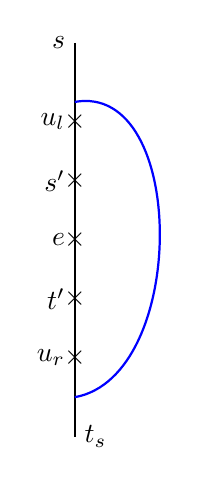
\begin{tikzpicture}[scale=1]

\coordinate (x) at (0,5);
\coordinate (y) at (0,0);
\coordinate (u) at (0,2.5);
\coordinate (ul) at (0,1);
\coordinate (ur) at (0,4);

\coordinate (x1) at (0,1.75);
\coordinate (y1) at (0,3.25);

\draw[thick](x)--(y);
\node[left] at (x){$s$};
\node[right] at (y){$t_{s}$};

\node[left] at (u){$e$};
\node at (u){$\times$};
\node[left] at (ul){$u_r$};
\node at (ul){$\times$};
\node[left] at (ur){$u_l$};
\node at (ur){$\times$};

\node[left] at (x1){$t'$};
\node at (x1){$\times$};
\node[left] at (y1){$s'$};
\node at (y1){$\times$};

\draw[thick,blue] (0,0.5) to[out=10,in=10] node[pos=0.2,
left]
{ } (0,4.25);
\end{tikzpicture}
\caption{The hardest part of the distance oracle, when the
replacement path neither passes through $u_l$ not $u_r$.}
\end{figure}

\noindent   Assume that we get a query
{\sc Q}($s,t,e(u,v)$), that is, find the shortest path from
$s$ to $t$ avoiding $e$. Assume without loss of generality that $u$ is closer to $s$ on $st$ path than $v$. We answer this query as follows:
first we find the distance of $v$ from $s$, via $B_0(s,v)$. If $B_0(s,v)$ is a power of 2 then
we can directly use $B_3(s,t_s, \oplus |sv|) + B_0(t_s,t)$. Else, let $u_l \leftarrow  B_2(s,v)$ and
$u_r \leftarrow B_2(t_s,u)$. Here $u_l$ is the nearest vertex to $s$ on $vs$ path whose
 distance from $v$ is a power of 2. Similarly, $u_r$ is the nearest vertex to $t_s$ on $ut_s$ path whose distance form $u$ is a power of 2.    There are three cases now:

\begin{enumerate}[noitemsep,nolistsep]
\item  The  preferred replacement path passes through $u_l$.

\item  The preferred replacement path passes through $u_r$.

\item The preferred replacement path neither passes through $u_l$
nor $u_r$.

\end{enumerate}
\noindent For the first case, we  can report $B_0(s,u_l) + B_3(u_l, t_{s}, \oplus|u_lv|) + B_0(t_s,t) $. For the second case, we can report $B_4(s,u_r, \ominus  |uu_r|) + B_0(u_r,t_s) + B_0(t_s,t)$ . The hardest
case is when the preferred replacement path neither passes through
$u_l$ nor $u_r$. Let $s'$ be the farthest
vertex  on $sv$ path from $s$ whose distance is a power
of 2, that is $|ss'| = 2^{\lfloor \log |sv| \rfloor}$. Similarly let $t'$ be the farthest vertex on $t_{s}u$
path from $t_s$ whose distance is a power
of 2. Now,
we can  report the shortest path from $s$ to $t_{s}$ avoiding
$[s',t']$ -- this is also stored in $B_5(s,t_s,[\oplus 2^{\lfloor \log |sv| \rfloor}, \ominus 2^{\lfloor
\log |t_su| \rfloor}] )$. By construction, if the shortest path avoids $[u_l,u_r]$, then it also
avoids $[s',t']$. Thus we can return $B_5(s,t_s,[\oplus 2^{\lfloor \log |sv| \rfloor}, \ominus 2^{\lfloor
\log |t_su| \rfloor}] ) +\ B_0(t_s,t)$ as the length  of the preferred replacement path.
The reader can check that the running time of our algorithm
is $O(1)$ as we have to check $B_0,B_1,B_2,B_3,B_4,B_5$ constant number of times.
For the correctness of the above procedure, please refer to \cite{DemetrescuTCR08,DuanP09}.
\else
Since this case is a generalization of the techniques developed by
Demetrescu et. al. \cite{DemetrescuTCR08}, concerned reader may read
the full version of the paper for details -- where we show that there exists a data-structure
of size $\tilde O(\sigma^{1/2}n^{3/2})$ which takes $O(1)$ time to find a replacement
path from $s$ to $t$ that avoids $e$ but passes through $t_s$.
\fi

Now, we move on to the harder case, that is, replacement paths avoid $t_s$ too. For this, we will  fix a vertex $t$. We will show
that the query
${\sc Q}(s,t,e(u,v))$  can be answered
in $\tilde O(1)$ using $\tilde O(\sqrt{\sigma n})$ space.
This immediately implies that we can answer exact queries
in $\tilde O(1)$ time using $\tilde O(\sigma^{1/2} n^{3/2})$
space.

%In the rest of the paper, we try to find a distance
%oracle for a fixed $t$.

% !TEX root = paper.tex
\iflong
\else
\vspace{-2mm}
\fi
\section{Preferred Replacement path avoids $t_s$}

\label{sec:avoids}


Handling preferred replacement paths that avoid $t_s$ turns out to be a challenging and unexplored case. For better exposition, we will first solve the problem for the case when $\sigma=1$, that is there is only one source.
Let $\RR$ be the set of all preferred replacement paths from $s$ to $t$ that do not pass through $t_s$. We make  two important observations:

\begin{enumerate}[noitemsep,nolistsep]

\item The size of $\RR$ is $ O(\sqrt n)$.

\item Preferred replacement paths in $\RR$ avoid one contiguous sub path of $st$.

\end{enumerate}

\noindent Few remarks are in order. If the preferred replacement paths in $\RR$ were disjoint, then bounding the size of $\RR$ is easy. However, we are able to bound the size of $\RR$ even if paths are intersecting.  The second observation implies that we can build a balanced binary search tree containing paths in $\RR$. Each node in this tree will contain a preferred replacement path $P$. The key for each node will be the start and end vertex of the sub path $P$ avoids.  We will use this BST to find an appropriate replacement path that avoids an edge $e$.

\begin{definition}(Detour of a replacement path)
Let $P$ be a preferred replacement path avoiding an edge $e$ on $st$ path. Then detour of $P$ is defined as, $\DET(P) := P \setminus st$. That is, detour is a path the leaves $st$ before $e$ till the point it merges back to $st$ again.
\end{definition}

\begin{comment}
\begin{lemma}
\label{lem:prop}
Let $P$ be a replacement path in $\RR$ that avoids $u$ on $st_s$ path. Then
 $P$ can merge back to $st$ path just once.
\end{lemma}
\begin{proof}
Since $P$ is a replacement path from $s$ to $t$ avoiding $u$, it necessary has to merge somewhere on path $st$. Assume that $P$ merges back at $w$ on $st$ path. Note that $w$ cannot lie before $u$ on $st$ path as the sub-path $sw$ of the $st$ path is the shortest path from $s$ to $w$. This implies that $w$ lies after $u$ on $st$ path. After merging at $w$, $P$ can continue on the sub path $wt$ (of path $st$) to reach $t$, as this is the shortest path from $w$ to $t$.
\end{proof}
\end{comment}
\noindent Since our  replacement path $P$  also avoids $t_s$, the following lemma is immediate by the definition of preferred path.

\begin{lemma}
Let $P$ be a preferred replacement path in $\RR$ that avoids $e$ and $t_s$ on
$st$ path, then (1) $\DET(P)$ cannot merge back to $st_s$ path and (2) $\DET(P)$ is a contiguous path.
\end{lemma}
\begin{lemma}
\label{lem:avoids}
Let $P,P' \in \RR$ avoid $e$ and $e'$ respectively on $st_s$ path. Also assume that $e$ is closer to $s$ than $e'$. Then
(1)  P avoids $e'$  (2) $\DET(P')$ starts  after $e$ on $st_s$ path and (3) $|P| > |P'|$.

\end{lemma}

\iflong
  \begin{proof}

  \noindent (1) $P$ diverges from $st_s$ path above $e$. Since $P
  \in \RR$, it   merges back on $t_st$ path only. Since $e,e'
  \in st_s$ (we are in {\em far} case) and $e$ is closer to $s$ than $e'$, this implies
  that $P$ also avoids $e'$.

  \noindent (2) Assume that  $\DET(P')$ starts above $e$ on
  $st_s$ path. This implies that both $P$ and $P'$ avoid $e$
  and $e'$. But then, our algorithm will choose one of these two paths as a preferred path that avoids both $e$ and $e'$.  Thus,
  we arrive at a contradiction as there are two different preferred replacement paths avoiding $e$ and $e'$.

  \noindent (3) Since $P$  avoids $e'$ (by (1)) and $\DET(P')$ starts after $e$ (by (2)), $P'$ is the preferred path to avoid $e'$ only if $|P'| < |P|$ (else $P$ would be the preferred path as it leaves the $st$ path earlier than $P'$).



  \end{proof}
\fi

\noindent The converse of the third part of the lemma is also true. Since we will be using it in future, we prove it now.

\begin{lemma}
\label{lem:avoidreverse}

Let   $P$ and $P'$ be two preferred replacement paths that avoid $e$ and $e'$ on $st$ path respectively. If $|P| > |P'|$, then $e$ is closer to $s$ than $e'$.
\end{lemma}

\iflong
  \begin{proof}
  Assume for contradiction that $e'$ is closer to $s$ than $e$. Since the replacement path $P'$ has to diverge from $st$ before $e'$ and merge again only in $t_st$,  $P'$ also avoid $e$. But then $P'$ should be the replacement path for avoiding $e$ too, as $|P'| < |P|$, a  contradiction.
  \end{proof}
\fi
\iflong
\else
\begin{figure}[hpt!]
\centering
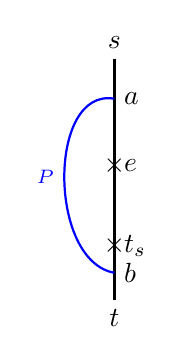
\begin{tikzpicture}[scale=1.7]

\definecolor{dgreen}{rgb}{0.0, 0.5, 0.0}
\begin{scope}[xshift=0cm]
\coordinate (s) at (0,1.8);
\coordinate (t) at (0,0);
\coordinate (ts) at (0,0.4);
\coordinate (b) at (0,.2);

\coordinate (a) at (0,1.5);
\coordinate (v) at (0,1);

\draw[thick](s)--(t);
\node[above] at (s){$s$};
\node[below] at (t){$t$};
\node[right] at (a){$a$};
\node[right] at (b){$b$};



\draw[blue,thick] (a) to[out=170,in=170] node[pos=0.5,left]
{\scriptsize  $P$}  (b);
\node at (v){$\times$};
\node[right] at (v){$e$};

\node at (ts){$\times$};
\node[right] at (ts){$t_s$};
\end{scope}

\end{tikzpicture}

\caption{$\DET(P)$ does not intersect detour of any path in $(>P)$}
\label{fig:singlefirstcase}
\end{figure}

\fi
\noindent By Lemma \ref{lem:avoids}{\small(3)}, we know that all preferred replacement
paths in $\RR$ have different lengths. In fact, it is the main reason we defined a preferred replacement path. We can thus arrange
these paths   in decreasing order of their lengths. Thus, we get the following corollary.
\begin{corollary}
\label{cor:arrange}
 Given a set $\RR$ of preferred replacement paths from $s$ to $t$ (that also avoid $t_s$), we can arrange  paths in decreasing order of their lengths.
\end{corollary}

\noindent Given a path $P \in \RR$, let $(<P)$ be the set of all preferred replacement paths with length less than $P$. Similarly, let $(>P)$ be the set of all preferred replacement paths with length greater than $P$.   If $P$ avoids $e$, then by Lemma \ref{lem:avoidreverse}, it also avoids all  edges avoided by paths in $(<P)$.  By Lemma \ref{lem:avoids}, for any path $P' \in (<P)$, $\DET(P')$ starts after $e$ on $st_s$ path.
We will now show a simple but important property of a path $P$ in $\RR$.

\begin{lemma}
\label{lem:length}
Let $P \in \RR$ be the shortest path from $s$ to $t$ avoiding $e$ such that $|P| = |st| +\ \ell$ where $\ell \ge 0$, then the size of the set $(<P)$ is $\le \ell$.
\end{lemma}
\iflong
  \begin{proof}
  Since a path in $(<P)$ avoids some edge in $st$ path, its length has to be $\ge |st|$. By Corollary \ref{cor:arrange},
  all paths in $\RR$, and thus $(<P)$ have different lengths. But the length of paths in $(<P)$ is less than the length of $P$.
  Thus, there can be atmost $\ell$ paths in $(<P)$.
  \end{proof}
\fi

\begin{definition}
\label{def:unique}
(Unique path of $P$) Let $\UNQ(P)$ be the prefix of\ $\DET(P)$ which does not intersect with any detours in $\cup_{P' \in (>P)} \DET(P')$.
\end{definition}
%Note that $\UNQ(P)$ can be an empty path too.
We now arrange all  preferred replacement paths in $\RR$ in decreasing order of their lengths. Assume that we are processing a path $P$ according to this ordering such that $P$ avoids $e$ on $st$ path. If $|\UNQ(P)| \ge \sqrt n$, then we have associated $O(\sqrt n)$ vertices on $\UNQ(P)$ to $P$. Else $\UNQ(P) < \sqrt{n}$ and we have the following two cases:

\iflong
\else
\vspace{-2mm}
\fi
\subsection{   $\DET(P)$ does not intersect with  detour of any path in $(>P)$}
\label{subsec:singlecaseone}
\iflong
\begin{figure}[hpt!]
\centering
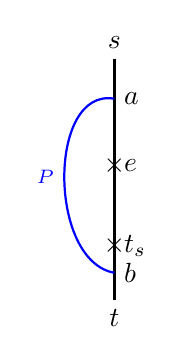
\begin{tikzpicture}[scale=1.7]

\definecolor{dgreen}{rgb}{0.0, 0.5, 0.0}
\begin{scope}[xshift=0cm]
\coordinate (s) at (0,1.8);
\coordinate (t) at (0,0);
\coordinate (ts) at (0,0.4);
\coordinate (b) at (0,.2);

\coordinate (a) at (0,1.5);
\coordinate (v) at (0,1);

\draw[thick](s)--(t);
\node[above] at (s){$s$};
\node[below] at (t){$t$};
\node[right] at (a){$a$};
\node[right] at (b){$b$};



\draw[blue,thick] (a) to[out=170,in=170] node[pos=0.5,left]
{\scriptsize  $P$}  (b);
\node at (v){$\times$};
\node[right] at (v){$e$};

\node at (ts){$\times$};
\node[right] at (ts){$t_s$};
\end{scope}

\end{tikzpicture}

\caption{$\DET(P)$ does not intersect detour of any path in $(>P)$}
\label{fig:singlefirstcase}
\end{figure}

\fi
    Let $\DET(P)$ start at $a$ and end at $b$ -- the vertex where it touches
    $t_st$ path. Let $ab$ denote the
path from $a$ to $b$ on $P$. By our assumption $\UNQ(P) = ab$ and $|ab| < \sqrt n$.
    By Lemma \ref{lem:avoids}, all  replacement paths in $(<P)$ pass through $e$
    (as detour of these replacement paths start below $e$) and by Lemma \ref{lem:avoidreverse},
    these replacement paths avoid edges that are closer to $t$ than $e$. We can view the
    replacement paths as if they are starting from the vertex $a$. That is, consider  paths
    $\{P\setminus sa\} \cup \{ P'\setminus sa | \ P' \in (<P)\}$. These replacement
    paths avoid edges in $at$.   $|P \setminus sa| = |ab| +  |bt| \le |ab|\ + |at| < |at| + \sqrt n$.
    Applying Lemma \ref{lem:length}, we infer that the number of paths in $\{ P'\setminus
sa | P' \in (<P)\}$ is $\le \sqrt n$

\iflong
\else
\vspace{-2mm}
\fi
\subsection{$\DET(P)$ intersects with  detour of a path in $(>P)$}
\label{subsec:singlecasetwo}
Assume that $P$ first intersects with $P' \in (>P)$. Let $P'$ avoid $e'$ and $\DET(P')$ start at $a'$ and end at $b'$ (see Figure \ref{fig:singlesecondcase}). Let us assume that $\DET(P)$ starts at $a$ and it intersects $\DET(P')$ at $c$. This implies that $\UNQ(P) = ac$.

\noindent Consider the path $sa' \conc a'c \conc ca \conc at$. We claim that this path avoids $e'$. This is due to the fact that by Lemma \ref{lem:avoids}, $\DET(P)$
starts after $e'$ on $st$ path. So, $ca$ and $at$ avoids $e'$. Since $P' = sa' \conc a'c \conc cb' \conc b't$, length of $P'$ must be $\le$ length of the alternate path. Thus,\\
\begin{tabular}{llll}
 & $|sa'| +  |a'c|
+ |cb'| + |b't|$  & $\le$ &$|sa'| + |a'c| + |ca|  + |at|$\\
$\implies$& $
|cb'| + |b't|$ & $\le$ & $|ca|  + |at|$   \\
$\implies$& $|ac| +
|cb'| + |b't|$ & $\le$ &   $2|ca|  + |at|$

\end{tabular}

\begin{figure}[hpt!]
\centering
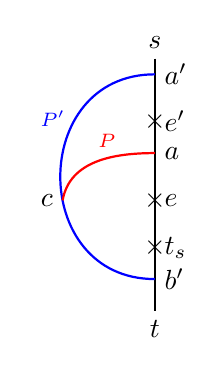
\begin{tikzpicture}[scale=2]

\definecolor{dgreen}{rgb}{0.0, 0.5, 0.0}
\begin{scope}[xshift=0cm]
\coordinate (s) at (0,1.6);
\coordinate (t) at (0,0);
\coordinate (ts) at (0,0.4);
\coordinate (b1) at (0,.2);

\coordinate (a1) at (0,1.5);
\coordinate (a) at (0,1);
\coordinate (v) at (0,0.7);
\coordinate (v1) at (0,1.2);
\coordinate (c) at (-0.585,0.7);

\draw[thick](s)--(t);
\node[above] at (s){$s$};
\node[below] at (t){$t$};
\node[right] at (a1){$a'$};
\node[right] at (a){$a$};
\node[right] at (b1){$b'$};
\node[left] at (c){$c$};


\draw[blue,thick] (a1) to[out=180,in=180,distance=.8cm] node[pos=0.3,left]
{\scriptsize  $P'$}  (b1);

\draw[red,thick] (a) to[out=180,in=80]
node[pos=0.4,above]
{\scriptsize  $P$}  (c);

\node at (v1){$\times$};
\node[right] at (v1){$e'$};

\node at (v){$\times$};
\node[right] at (v){$e$};

\node at (ts){$\times$};
\node[right] at (ts){$t_s$};
\end{scope}

\end{tikzpicture}

\caption{$\DET(P)$ intersects first with $\DET(P')$ at $c$ where  $P'
\in (>P)$.}
\label{fig:singlesecondcase}
\end{figure}

On the left hand of the inequality, we  have a path from $a$ to $t$ avoiding $e$. So, its length should be $\ge$ length of the preferred path $P \setminus sa$. Thus $|P \setminus sa| \le  2|ca|  + |at| \le 2\sqrt n\
+\ |at|$. By Lemma \ref{lem:avoids},
all  replacement paths in $(<P)$ pass through $e$ (as
detour of these replacement paths start below $e$) and by
Lemma \ref{lem:avoidreverse}, these replacement paths avoid
edges that are closer to $t$ than $e$. We can view the
replacement paths as if they are starting from the vertex $a$.
That is, consider  paths $\{P\setminus sa\} \cup \{ P'\setminus
sa | P' \in (<P)\}$. Applying lemma \ref{lem:length}, we infer that the number of
paths in $\{ P'\setminus
sa | P' \in (<P)\}$ is $\le 2 \sqrt n$.


Our arguments above point to the following important observation: {\em Once we find a replacement path in $\RR$ with unique path length $< \sqrt n$, then there are at most 2$\sqrt n$ replacement paths in $\RR$ left to process.}
Since there can be at most $\sqrt n$ paths in $\RR$ with unique path length $\ge \sqrt n$, we have proven the following lemma:

\begin{lemma}
\label{lem:sizeR}
%Let $\RR$ be all the replacement paths from $s$ to $t$ whose detour avoids $t_s$, then
$|\RR| = O(\sqrt n)$.
\end{lemma}

We now build a data-structure which will exploit Lemma \ref{lem:sizeR}.
However, we need another key but simple observation. By Lemma \ref{lem:avoids}, if $|P| > |P'|$, then $\DET(P')$ starts below the edge avoided by $P$. This lemma implies that $\DET(P')$ starts below all  edges avoided by $P$. Thus $P$ avoids some contiguous path in $st_s$ and detour of all replacement paths in $(<P)$ start below the last edge (which is closer to $t_s$) in this subpath. Thus, we have proved the second key lemma:

\begin{lemma}
\label{lem:contiguous}

A replacement path $P$ avoids a contiguous subpath of $st$.
\end{lemma}
\iflong
\else

\begin{figure}[hpt!]

\centering
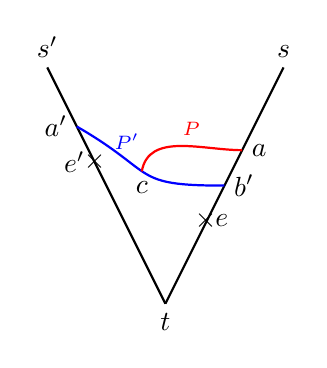
\begin{tikzpicture}[scale=1.5]

\definecolor{dgreen}{rgb}{0.0, 0.5, 0.0}
\begin{scope}[xshift=0cm]
\coordinate (s) at (-1,2);
\coordinate (s1) at (1,2);
\coordinate (t) at (0,0);
\coordinate (ts) at (0,0.4);
\coordinate (b1) at (0.5,1);

\coordinate (a1) at (-0.75,1.5);
\coordinate (a) at (0.65,1.3);
\coordinate (v) at (0.34,0.7);
\coordinate (v1) at (-0.6,1.2);
\coordinate (c) at (-0.2,1.12);

\draw[thick](s)--(t);
\draw[thick](s1)--(t);
\node[above] at (s){$s'$};
\node[above] at (s1){$s$};
\node[below] at (t){$t$};
\node[left] at (a1){$a'$};
\node[right] at (a){$a$};
\node[right] at (b1){$b'$};
\node[below] at (c){$c$};


\draw[blue,thick] (a1) to[out=330,in=180,distance=.8cm]
node[pos=0.3,above]
{\scriptsize  $P'$}  (b1);

\draw[red,thick] (a) to[out=180,in=80]
node[pos=0.4,above]
{\scriptsize  $P$}  (c);

\node at (v1){$\times$};
\node[left] at (v1){$e'$};

\node at (v){$\times$};
\node[right] at (v){$e$};

\end{scope}

\end{tikzpicture}

\caption{The bad case for us: $P' \in (>P)$ intersects with $P$ and then passes through the edge $e$ that $P$ avoids. }
\label{fig:multiple}
\end{figure}

\fi
Let $\FF(P)$ and $\LL(P)$ denote the first and the last vertex of the contiguous path that $P$ avoids. Given a vertex $v$, let $v.depth$ denote the depth of $v$ in the BFS tree of $s$.  We can store the depth of all  vertices in an array (takes $O(n)$ space). Lastly, we build a balanced binary search tree\ BST($t$) in which each node represents a path $P$. The key used to search the node is the range: $[\FF(P).depth, \LL(P).depth]$. By Lemma \ref{lem:contiguous}, all  replacement paths avoid  contiguous subpaths of $st_s$.  These contiguous paths are also disjoint as there is only one preferred path avoiding an edge. Thus, the key we have chosen forms a total ordered set with respect to the relation $\{ <,>\}$.  The size of BST($t$) is $O(\sqrt n)$ as the size of $\RR$ is $O(\sqrt n)$. We are now ready to process any query {\sc Q}$(s,t,e(u,v))$. We just need to search for an interval in BST($t$) that contains $u.depth$ and $v.depth$. This can be done in $\tilde O(1)$ time. Thus we have proved the following theorem:

\begin{theorem}
There exists a data-structure of size $\tilde O(n^{3/2})$ for single source single fault tolerant exact distance oracle that can answer each query in $\tilde O(1)$ time.
\end{theorem}


We briefly recall the framework of statistical inference via empirical risk minimization.
Let $(\bbZ, \calZ)$ be a measurable space.
Let $Z \in \bbZ$ be a random element following some unknown distribution $\Prob$.
Consider a parametric family of distributions $\calP_\Theta := \{P_\theta: \theta \in \Theta \subset \reals^d\}$ which may or may not contain $\Prob$.
We are interested in finding the parameter $\theta_\star$ so that the model $P_{\theta_\star}$ best approximates the underlying distribution $\Prob$.
For this purpose, we choose a \emph{loss function} $\score$ and minimize the \emph{population risk} $\risk(\theta) := \Expect_{Z \sim \Prob}[\score(\theta; Z)]$.
Throughout this paper, we assume that
\begin{align*}
     \theta_\star = \argmin_{\theta \in \Theta} L(\theta)
\end{align*}
uniquely exists and satisfies $\theta_\star \in \text{int}(\Theta)$, $\nabla_\theta L(\theta_\star) = 0$, and $\nabla_\theta^2 L(\theta_\star) \succ 0$.

\myparagraph{Consistent loss function}
We focus on loss functions that are consistent in the following sense.

\begin{customasmp}{0}\label{asmp:proper_loss}
    When the model is \emph{well-specified}, i.e., there exists $\theta_0 \in \Theta$ such that $\Prob = P_{\theta_0}$, it holds that $\theta_0 = \theta_\star$.
    We say such a loss function is \emph{consistent}.
\end{customasmp}

In the statistics literature, such loss functions are known as proper scoring rules \citep{dawid2016scoring}.
We give below two popular choices of consistent loss functions.

\begin{example}[Maximum likelihood estimation]
    A widely used loss function in statistical machine learning is the negative log-likelihood $\score(\theta; z) := -\log{p_\theta(z)}$ where $p_\theta$ is the probability mass/density function for the discrete/continuous case.
    When $\Prob = P_{\theta_0}$ for some $\theta_0 \in \Theta$,
    we have $L(\theta) = \Expect[-\log{p_\theta(Z)}] = \kl(p_{\theta_0} \Vert p_\theta) - \Expect[\log{p_{\theta_0}(Z)}]$ where $\kl$ is the Kullback-Leibler divergence.
    As a result, $\theta_0 \in \argmin_{\theta \in \Theta} \kl(p_{\theta_0} \Vert p_\theta) = \argmin_{\theta \in \Theta} L(\theta)$.
    Moreover, if there is no $\theta$ such that $p_\theta \txtover{a.s.}{=} p_{\theta_0}$, then $\theta_0$ is the unique minimizer of $L$.
    We give in \Cref{tab:glms} a few examples from the class of generalized linear models (GLMs) proposed by \citet{nelder1972generalized}.
\end{example}

\begin{example}[Score matching estimation]
    Another important example appears in \emph{score matching} \citep{hyvarinen2005estimation}.
    Let $\bbZ = \reals^\tau$.
    Assume that $\Prob$ and $P_\theta$ have densities $p$ and $p_\theta$ w.r.t the Lebesgue measure, respectively.
    Let $p_\theta(z) = q_\theta(z) / \Lambda(\theta)$ where $\Lambda(\theta)$ is an unknown normalizing constant. We can choose the loss
    \begin{align*}
        \score(\theta; z) := \Delta_z \log{q_\theta(z)} + \frac12 \norm{\nabla_z \log{q_\theta(z)}}^2 + \text{const}.
    \end{align*}
    Here $\Delta_z := \sum_{k=1}^p \partial^2/\partial z_k^2$ is the Laplace operator.
    Since \cite[Thm.~1]{hyvarinen2005estimation}
    \begin{align*}
        L(\theta) = \frac12 \Expect\left[ \norm{\nabla_z q_\theta(z) - \nabla_z p(z)}^2 \right],
    \end{align*}
    we have, when $p = p_{\theta_0}$, that $\theta_0 \in \argmin_{\theta \in \Theta} L(\theta)$.
    In fact, when $q_\theta > 0$ and there is no $\theta$ such that $p_\theta \txtover{a.s.}{=} p_{\theta_0}$, the true parameter $\theta_0$ is the unique minimizer of $L$ \cite[Thm.~2]{hyvarinen2005estimation}.
\end{example}

\myparagraph{Empirical risk minimization}
Assume now that we have an i.i.d.~sample $\{Z_i\}_{i=1}^n$ from $\Prob$.
To learn the parameter $\theta_\star$ from the data, we minimize the empirical risk to obtain the \emph{empirical risk minimizer}
\begin{align*}
    \theta_n \in \argmin_{\theta \in \Theta} \left[ L_n(\theta) := \frac1n \sum_{i=1}^n \score(\theta; Z_i) \right].
\end{align*}
This applies to both maximum likelihood estimation and score matching estimation. 
In \Cref{sec:main_results}, we will prove that, with high probability, the estimator $\theta_n$ exists and is unique under a generalized self-concordance assumption.

\begin{figure}
    \centering
    \includegraphics[width=0.45\textwidth]{graphs/logistic-dikin} %0.4
    \caption{Dikin ellipsoid and Euclidean ball.}
    \label{fig:logistic_dikin}
\end{figure}

\myparagraph{Confidence set}
In statistical inference, it is of great interest to quantify the uncertainty in the estimator $\theta_n$.
In classical asymptotic theory, this is achieved by constructing an asymptotic confidence set.
We review here two commonly used ones, assuming the model is well-specified.
We start with the \emph{Wald confidence set}.
It holds that $n(\theta_n - \theta_\star)^\top H_n(\theta_n) (\theta_n - \theta_\star) \rightarrow_d \chi_d^2$, where $H_n(\theta) := \nabla^2 L_n(\theta)$.
Hence, one may consider a confidence set $\{\theta: n(\theta_n - \theta)^\top H_n(\theta_n) (\theta_n - \theta) \le q_{\chi_d^2}(\delta) \}$ where $q_{\chi_d^2}(\delta)$ is the upper $\delta$-quantile of $\chi_d^2$.
The other is the \emph{likelihood-ratio (LR) confidence set} constructed from the limit $2n [L_n(\theta_\star) - L_n(\theta_n)] \rightarrow_d \chi_d^2$, which is known as the Wilks' theorem \citep{wilks1938large}.
These confidence sets enjoy two merits: 1) their shapes are an ellipsoid (known as the \emph{Dikin ellipsoid}) which is adapted to the optimization landscape induced by the population risk; 2) they are asymptotically valid, i.e., their coverages are exactly $1 - \delta$ as $n \rightarrow \infty$.
However, due to their asymptotic nature, it is unclear how large $n$ should be in order for it to be valid.

Non-asymptotic theory usually focuses on developing finite-sample bounds for the \emph{excess risk}, i.e., $\Prob(L(\theta_n) - L(\theta_\star) \le C_n(\delta)) \ge 1 - \delta$.
To obtain a confidence set, one may assume that the population risk is twice continuously differentiable and $\lambda$-strongly convex.
Consequently, we have $\lambda \norm{\theta_n - \theta_\star}_2^2 / 2 \le L(\theta_n) - L(\theta_\star)$ and thus we can consider the confidence set $\calC_{\text{finite}, n}(\delta) := \{\theta: \norm{\theta_n - \theta}_2^2 \le 2C_n(\delta)/\lambda\}$.
Since it originates from a finite-sample bound, it is valid for fixed $n$, i.e., $\Prob(\theta_\star \in \calC_{\text{finite}, n}(\delta)) \ge 1 - \delta$ for all $n$; however, it is usually conservative, meaning that the coverage is strictly larger than $1 - \delta$.
Another drawback is that its shape is a Euclidean ball which remains the same no matter which loss function is chosen.
We illustrate this phenomenon in \Cref{fig:logistic_dikin}.
Note that a similar observation has also been made in the bandit literature \citep{faury2020improved}.

We are interested in developing finite-sample confidence sets.
However, instead of using excess risk bounds and strong convexity, we construct in \Cref{sec:main_results} the Wald and LR confidence sets in a non-asymptotic fashion, under a generalized self-concordance condition.
These confidence sets have the same shape as their asymptotic counterparts while maintaining validity for fixed $n$.
These new results are achieved by characterizing the critical sample size enough to enter the asymptotic regime.

% !TEX root = paper.tex
\begin{comment}
\section{Analysing preferred paths in $\TZE$}
For each segment $xy$ in \SBFS$(t)$ (with $y$ closer to $t$ than $x$),
we store the shortest path from $x$ to $t$ avoiding vertex $y$ (and $t_x$)
in $\TZE(xy)$. Note that the size of $|\ \{ \TZE(xy) |\ xy \ \text{is a segment in \SBFS($t$)} \}|$
is $O(\sigma) = O(\sqrt{n \sigma})$.

However, this data-structure in itself will not be able to answer query
$\QQ(s,t,u)$ where $u$ is an intersection point. We will expand  say
more on this issue in the next section.
\end{comment}
%By definition, \SBFS$(t)$ has $O(\sigma)$ intersection vertices. So, we can
%store the preferred replacement path that avoid these intersection vertices
%in a balaced binary search tree $\BST_1(t)$. In Section \ref{sec:data},
%we will see how to use this data-structure.
%Given a query $\textsc{Q}(s,t,u)$,
%we first check if $u$ is an intersection vertex in \SBFS$(t)$. If yes, in $\tilde O(1)$
%time, we return the preferred replacement path corresponding to the intersection
%vertex $u$. The space taken by $\BST_1(t)$ is $O(\sigma) = O(\sqrt{n \sigma})$.

\iflong
\else
\vspace{-2mm}
\fi
\section{Analysing preferred replacement paths in $\TON$}
\label{sec:multi1}
We first show the following:
\begin{lemma}
\label{lem:allsame}
For each segment $xy \in$ \SBFS$(t)$, $|\TON(xy)| = 1$
\end{lemma}
\iflong
\begin{proof}
  %Let $t_x$ be the vertex in $\TT$ closest to
  %$t$ on $xt$ path. Remember that we are looking at the case
  %when the replacement path avoids $t_x$, that is, the replacement
  %path merges back on $t_xt$ path.
  Assume that there are two preferred paths
   $P$ and $P'$ whose detour start in $xy$ and their avoided edge $e$ and
  $e'$(respectively) lie in $yt_x$. Since we are analyzing
  paths in the {\em far case},  detours of $P$ and $P'$ meet $xt$ path in $t_xt$ subpath.
  Since both $e$ and $e'$ lie on $yt_x$ path,
  this implies that both $P$ and $P'$ avoid $e$ and $e'$.
  Thus, we will choose the smaller of the two paths as the preferred path avoiding both
  $e$ and $e'$. Else if $|P| = |P'|$, then we will choose that path which leaves the $xt$
  path as early as possible. Thus, there is only one preferred path avoiding both
  $e$ and $e'$, a contradiction.
  \end{proof}
\fi

%Viewed from the vantage point of intersection vertex $x$, the above lemma implies that
%there is no difference between preferred path (in $\TON$) whose detour start in $xy$.
%This is due to the fact that suffix of these path are same once they hit $x$.
%So, we only need to store this common suffix (starting from $x$) for paths in $\TON$ per segment.
%We will exploit this feature of $\TON$ when we build our data-structure in Section \ref{sec:data}
%Let $\TON(xy)$ denote the preferre replacement path from $x$ to $t$ which avoids all
%edges in $yt_x$. Note that the size of $|\{ \TON(xy) |\ xy \ \text{is a segment in \SBFS($t$)} \}|$
\noindent The above lemma implies that $|\TON| = \cup_{xy \in \text{\SBFS($t$)}} |\TON(xy)| =
O(\sigma) = O(\sqrt{n \sigma})$.
%We will see that this data-structure in itself will not be able to answer query
%$\QQ(s,t,e)$. We will defer this discussion till the next section.




%\section{Discussion on Approximation \textit{vs} Stability and Recovery}\label{sec:approx-stability}


In the world of approximation algorithms, for a maximization problem for which an algorithm outputs $S$ and the optimum is $S^*$, what we typically try to prove is that
$w(S)\ge w(S^*)/\alpha$, even in the worst case; this \textit{approximation inequality} means that the algorithm at hand is an $\alpha$-approximation, so it is a \textit{good} algorithm. Though one might be quick to say that recovery of $\alpha$-stable instances immediately follows from the approximation inequality, this is not true because of the intersection $S\cap S^*$; if we have no intersection, then recovery indeed follows. 

What the research on stability and exact recovery suggests, is that we should try to understand if some of our already known approximation algorithms have the stronger property $w(S\setminus S^*)\ge w(S^*\setminus S)/\alpha$ or at least if they have it on stable instances. We refer to the latter as the \textit{recovery inequality}. This would directly imply an exact recovery result for $\alpha$-stable instances because we could $\alpha$-perturb only the $S\setminus S^*$ part of the input and get: 
\[
\noindent w(S\setminus S^*)\ge w(S^*\setminus S)/\alpha \implies \alpha\cdot w(S\setminus S^*) +w(S\cap S^*) \ge w(S^*\setminus S) +w(S\cap S^*) = w(S^*)
\] thus violating the fact we were given an $\alpha$-stable instance, unless $S\setminus S^* = \emptyset$.

This would mean that the algorithm successfully retrieved $S^*$ and could potentially explain why many approximation algorithms behave far better in practice than in theory. Furthermore, from a theory perspective, it would mean that many results from the well-studied area of approximation algorithms could be translated in terms of stability and recovery.

As a concluding remark, we want to point out that even though one might think that an $\alpha$-approximation algorithm needs at least $\alpha$-stability for recovery, this is not true as the somewhat counterintuitive result from \cite{balcan2015k} tells us: asymmetric $k$-center cannot be approximated to any constant factor, but can be solved optimally on 2-stable instances. This was the
first problem that is hard to approximate to any constant factor in the worst case, yet can be optimally
solved in polynomial time for 2-stable instances. The other direction (having an $\alpha$-approximation algorithm that cannot recover arbitrarily stable instances) is also true. These findings suggest that there are interesting connections between stability, exact recovery and approximation.

\iflong
\else
\vspace{-2mm}
\fi
\section{Analysing preferred replacement paths in $\TTW$}
\label{sec:multi2}

%Let $xy$ be a segment in \SBFS($t$).
%Consider all the replacement that start in $xy$ and are in $\TTW$.
%Since we know that the detours of these path start in $xy$, (similar to $\TON$) we can view
%these replacement paths as if they are starting from $a$.

We first show that one special kind of path will never lie in $\TTW$.
This characterization will help in analyzing bad paths in $\TTW$.


\begin{lemma}
\label{lem:feature}
Let $P$ be a preferred path from $x$ to $t$ avoiding $e$ on $xt$ path.
If $P$ merges with any segment $x'y'$ and then diverges from $x't$ path, then $P \notin \TTW$.
\end{lemma}
\iflong
  \begin{figure}[hpt!]
\centering
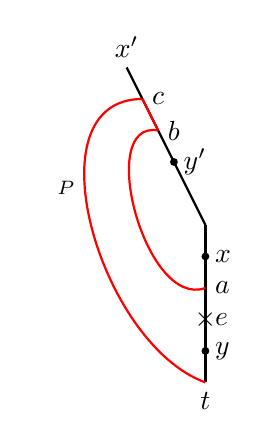
\begin{tikzpicture}[scale=2]
\begin{scope}
\coordinate (s) at (-0.5,2);
\coordinate (s1) at (0.5,2);
\coordinate (w) at (0,1);
\coordinate (t) at (0,0);
\coordinate (x) at (0,0.8);
\coordinate (y) at (0,0.2);
\coordinate (y1) at (-0.2,1.4);
\coordinate (i1) at (-0.4,1.8);
\coordinate (i2) at (-0.3,1.6);
\coordinate (a) at (0,0.6);
\coordinate (v) at (0,0.4);



\draw[thick](s)--(w);
%\draw[thick](s1)--(w);
\draw[thick](w)--(t);
\node[above] at (s){$x'$};
%\node[above] at (s1){$s$};
\node[below] at (t){$t$};

\node[right] at (a){$a$};

%\node[right] at (w){$w$};
\node[right] at (i1){$c$};
\node[right] at (i2){$b$};


\draw[red,thick] (a) to[out=200,in=170]
(i2);
\draw[red,thick](i1)--(i2);
\draw[red,thick] (i1) to[out=180,in=160]node[pos=0.4,left,black]{\scriptsize{$P$}}  (t);
\node at (v){$\times$};
\node[right] at (v){$e$};
\draw (y) node[fill,circle,scale=0.3]{};
\node[right] at (y){$y$};
\draw (x) node[fill,circle,scale=0.3]{};
\node[right] at (x){$x$};
\draw (y1) node[fill,circle,scale=0.3]{};
\node[right] at (y1){$y'$};
\end{scope}
\end{tikzpicture}
\caption{The path $P$ merges with another segment $x'y'$  and then diverges.}
\label{fig:feature}

\end{figure}

  \begin{proof}
  Once $P$ merges with $x'y'$ segment, it will diverge from it only if
  $x't$ contains $e$. This implies that $xt$ and $x't$ intersect or $xt$
  is a subpath of $x't$.
  %If $\DET(P)$ starts on $sw$ path
  %(before or on the intersection vertex $w$), then $P \in \TON$.
  %We will argue now that $\DET(P)$
  %cannot start after the intersection vertex.

  \noindent Assume for contradiction that $P \in \TTW$, that is, $\DET(P)$
  start strictly inside segment $xy$. Consider the Figure \ref{fig:feature} in which
  the detour of the preferred replacement path $P$
  starts after $x$ (at $a$). It then intersect  $x'y'$ at $b$
  and then diverges from $x't$ path at $c$.
  We claim that there exists another path to reach $b$ that is shorter  than
  $xa \conc ab$. This path is $xb$, where path $xb$ is a subpath of $x't$.
  It is also a shorter path (in $G_p$) as it uses
   edges in original $x't$ path.

  This path (1) diverges at $x$ and (2) is shorter (in $G_p$) as it uses edges from $x't$ path.
  Thus, there is a shorter replacement path than $P$ that avoids $e$. This path is not in
  $\TTW$ as its detour starts at $x$  .
  This leads to a contradiction as we had assumed that $P$ is the preferred replacement path avoiding $e$.
  Thus our assumption,
  namely that $P \in \TTW$ must be false.
  \end{proof}
\fi

\noindent We will now analyze  paths in $\TTW$. Consider two replacement
paths $P, P'$ avoiding edges $e,e'$ (respectively) on $xy,x'y'$ segment respectively.
%($ x,x'$  are intersection vertices in \SBFS($t$)) .
Let  $a,a'$ be the starting vertex of $\DET(P), \DET(P')$ respectively.
We say that $P \prec P'$ if $|at| < |a't|$.
If $|at| = |a't|$, then the tie is broken arbitrarily.


\noindent  Given a path $P \in \TTW$, let $(< P)$ be the set of all replacement
paths in $\TTW$ that are $\prec P$ in the ordering. Similarly, $(> P)$ is
the set of all replacement paths $P' \in \TTW$ for which $P \prec P'$.
Define $\UNQ(P)$ according to this ordering (see definition \ref{def:unique}).
Assume that we are processing a replacement path $P$ according to this ordering.
If $|\UNQ(P)| \ge \sqrt{n/\sigma}$, then we can associate $O(\sqrt{n/\sigma})$
{\em unique} vertices to $P$. Otherwise $|\UNQ(P)| < \sqrt{n/\sigma}$ and we have the following two cases:

\iflong
\else
\vspace{-2mm}
\fi



\subsection{ $\DET (P)$ does not intersect with any other detour in $(> P)$ }
\label{subsec:nointersect}
\noindent This case is similar to the first case in Section \ref{subsec:singlecaseone}.
\iflong
  Assume that $P$ avoids an edge $e$ on segment $xy$. Let $\DET(P)$
  start at $a \in xy$ and end at $b$ -- the vertex
  where it touches $t_xt$ path. Let $ab$ denote the
path from $a$ to $b$ on $P$. By our assumption $\UNQ(P)
  = ab$ and $|ab| < \sqrt{n/\sigma}$. Consider the following set
  of replacement paths  $(< P)_x := \{P' \in (< P)\ |\ P'~ \text{avoids an edge on $xy$ segment}\}$.
  By Lemma \ref{lem:avoids},
  all  replacement paths in $(< P)_x$ pass through $e$ (as
  detour of these replacement paths start below $e$) and by
  Lemma \ref{lem:avoidreverse}, these replacement paths avoid
  edges that are closer to $y$ than $e$. We can view these
  replacement paths as if they are starting from vertex $a$.
   $|P \setminus xa|
  = |ab| + |bt| \le \sqrt {n/\sigma} + |at|$. Using lemma \ref{lem:length}, total
  number of paths in   $(\le P)_x$ is  $\le \sqrt{ n/\sigma}$.  Thus, once we
  get a replacement path $P \in \TTW(xy)$ with $|\UNQ(P)| < \sqrt{n /\sigma}$, then there
  are at most $\sqrt{n/\sigma}$ replacement paths in $\TTW(xy)$ remaining to be processed.
  Thus, total number of paths in $\TTW$ with  $|\UNQ(P)|< \sqrt{n/\sigma}$ is
  $\sum_{xy \in \text{\SBFS($t$)}} \sqrt{n/ \sigma} = O(\sqrt{n \sigma})$
  (as there are $O(\sigma)$ segments in \SBFS($t$))
\else
   We can show that once we
   get a replacement path $P \in \TTW(xy)$ with $|\UNQ(P)| < \sqrt{n /\sigma}$, then there
   are at most $O(\sqrt{n/\sigma})$ replacement paths in $\TTW(xy)$ remaining to be processed. This will bound
   the total number of such paths to $O(\sqrt{n\sigma})$. Please see
   the full version for details.
\fi

\iflong
\else
\vspace{-2mm}
\fi
\subsection{ $\DET(P)$ intersects with  detour of a  path in $(> P)$}
\label{subsec:pintersects}

We first give a formal definition of a bad path that was defined informally in Section \ref{sec:problem}.
\begin{definition} (Bad Path)
A path $P \in \TTW$ is called a bad path if there exists another path $P' \in (>P)$
such that (1) $\DET(P)$ intersects with $\DET(P')$ and (2) $\DET(P')$ passes through the edge
avoided by $P$ after their intersection. We also say that $P$ is a bad replacement
path due to $P'$ if $P'$ satisfies the above two conditions.
\end{definition}

A path that is not bad is called a good path. In Section \ref{sec:problem}, we saw that
bad paths break the easy analysis of the single source case.
So, we have two cases depending on whether the path is good or bad. Let us look at the easier case first.\iflong\\\else\vspace{1mm}\fi


% Note that our analysis in Section \ref{sec:avoids} was easy as $P'$ cannot pass through $e$.
%However, as we have seen in Section \ref{sec:problem}, $P'$ can pass through $e$.
%Let us first look at the scenario when $P'$ does not pass through $e$ after intersection with $P$.
\iflong
\else
\section{Discussion on Approximation \textit{vs} Stability and Recovery}\label{sec:approx-stability}


In the world of approximation algorithms, for a maximization problem for which an algorithm outputs $S$ and the optimum is $S^*$, what we typically try to prove is that
$w(S)\ge w(S^*)/\alpha$, even in the worst case; this \textit{approximation inequality} means that the algorithm at hand is an $\alpha$-approximation, so it is a \textit{good} algorithm. Though one might be quick to say that recovery of $\alpha$-stable instances immediately follows from the approximation inequality, this is not true because of the intersection $S\cap S^*$; if we have no intersection, then recovery indeed follows. 

What the research on stability and exact recovery suggests, is that we should try to understand if some of our already known approximation algorithms have the stronger property $w(S\setminus S^*)\ge w(S^*\setminus S)/\alpha$ or at least if they have it on stable instances. We refer to the latter as the \textit{recovery inequality}. This would directly imply an exact recovery result for $\alpha$-stable instances because we could $\alpha$-perturb only the $S\setminus S^*$ part of the input and get: 
\[
\noindent w(S\setminus S^*)\ge w(S^*\setminus S)/\alpha \implies \alpha\cdot w(S\setminus S^*) +w(S\cap S^*) \ge w(S^*\setminus S) +w(S\cap S^*) = w(S^*)
\] thus violating the fact we were given an $\alpha$-stable instance, unless $S\setminus S^* = \emptyset$.

This would mean that the algorithm successfully retrieved $S^*$ and could potentially explain why many approximation algorithms behave far better in practice than in theory. Furthermore, from a theory perspective, it would mean that many results from the well-studied area of approximation algorithms could be translated in terms of stability and recovery.

As a concluding remark, we want to point out that even though one might think that an $\alpha$-approximation algorithm needs at least $\alpha$-stability for recovery, this is not true as the somewhat counterintuitive result from \cite{balcan2015k} tells us: asymmetric $k$-center cannot be approximated to any constant factor, but can be solved optimally on 2-stable instances. This was the
first problem that is hard to approximate to any constant factor in the worst case, yet can be optimally
solved in polynomial time for 2-stable instances. The other direction (having an $\alpha$-approximation algorithm that cannot recover arbitrarily stable instances) is also true. These findings suggest that there are interesting connections between stability, exact recovery and approximation.

\fi
\iflong\section{Discussion on Approximation \textit{vs} Stability and Recovery}\label{sec:approx-stability}


In the world of approximation algorithms, for a maximization problem for which an algorithm outputs $S$ and the optimum is $S^*$, what we typically try to prove is that
$w(S)\ge w(S^*)/\alpha$, even in the worst case; this \textit{approximation inequality} means that the algorithm at hand is an $\alpha$-approximation, so it is a \textit{good} algorithm. Though one might be quick to say that recovery of $\alpha$-stable instances immediately follows from the approximation inequality, this is not true because of the intersection $S\cap S^*$; if we have no intersection, then recovery indeed follows. 

What the research on stability and exact recovery suggests, is that we should try to understand if some of our already known approximation algorithms have the stronger property $w(S\setminus S^*)\ge w(S^*\setminus S)/\alpha$ or at least if they have it on stable instances. We refer to the latter as the \textit{recovery inequality}. This would directly imply an exact recovery result for $\alpha$-stable instances because we could $\alpha$-perturb only the $S\setminus S^*$ part of the input and get: 
\[
\noindent w(S\setminus S^*)\ge w(S^*\setminus S)/\alpha \implies \alpha\cdot w(S\setminus S^*) +w(S\cap S^*) \ge w(S^*\setminus S) +w(S\cap S^*) = w(S^*)
\] thus violating the fact we were given an $\alpha$-stable instance, unless $S\setminus S^* = \emptyset$.

This would mean that the algorithm successfully retrieved $S^*$ and could potentially explain why many approximation algorithms behave far better in practice than in theory. Furthermore, from a theory perspective, it would mean that many results from the well-studied area of approximation algorithms could be translated in terms of stability and recovery.

As a concluding remark, we want to point out that even though one might think that an $\alpha$-approximation algorithm needs at least $\alpha$-stability for recovery, this is not true as the somewhat counterintuitive result from \cite{balcan2015k} tells us: asymmetric $k$-center cannot be approximated to any constant factor, but can be solved optimally on 2-stable instances. This was the
first problem that is hard to approximate to any constant factor in the worst case, yet can be optimally
solved in polynomial time for 2-stable instances. The other direction (having an $\alpha$-approximation algorithm that cannot recover arbitrarily stable instances) is also true. These findings suggest that there are interesting connections between stability, exact recovery and approximation.
\fi

\noindent {(1) \em $P$ is a good path.}

\noindent Assume that $P \in \TTW(xy)$ and it avoids an edge $e \in xy$.
Assume that $P$  intersects first with $P' \in (> P)$ and $P'$ avoids $e'$ on $x'y'$ segment.
Note that $x$ may be equal to $x'$.
Let $\DET(P')$ start at $a'$ and end at
$b'$. Assume that $\DET(P)$ starts at $a$ and it intersects $\DET(P')$
at $c$.
Consider the path $x'a' \conc a'c \conc ca \conc at$. Since $x'a' \conc a'c$ is a part of $P'$,
it avoids $e'$. However, it is not clear whether $ca \conc at$ avoids $e'$ too.
In Figure \ref{fig:examples}, we see two representative examples in which $ca$ and $at$
avoid $e'$.
\iflong
  We will now show that both $ca$   and $at$ cannot passes through $e'$.
  %then $P$ is {\em similar} to $P'$
  %(in which case we can discard path $P$).
  \begin{enumerate}
   \item[(a)] Assume that  $ca$ passes through $e'$ %(See Figure \ref{fig:badexample1}(a))
    \label{enum:goodcase}

  If $x=x'$, then by Lemma \ref{lem:avoids}, as $P' \in (>P)$, $\DET(P)$ (and hence $ca$)
   starts below $e'$. Thus, $ca$ cannot pass through $e'$ as $\DET(P)$ does not
  intersect $xt_x$ path and $e' \in xt_x$. So let us assume that $x \neq x'$.
  This implies that $P$ intersects $x'y'$. After intersecting $x'y'$ path
    $P$ did not follow $x'y' \conc y't$ (since $ca$ intersect $\DET(P')$ at $c$).
    %This implies that $s't$ path contains $e$ (the vertex $P$ avoids).
    %Thus, $s't$ and $st$ intersect, say at $w$ and $e$ lies after $w$ on $s't$
    %and $st$ path. Since $P \in \TTW$, $\DET(P)$ should also start after $w$.
    %Since $\DET(P)$ passes through $e'$, $e'$ cannot lie on $wt$ path
    %(as $wt$ is a subpath of $st$ and by defintion $\DET(P)$ cannot intersect $st$).
    %Thus $e' \in sw$.
    This implies that $P$ intersect with another path $x'y'$ and then
    diverges. By Lemma \ref{lem:feature}, $P \notin \TTW$.
    This leads to a contradiction as we assumed that $P \in \TTW$. Thus our
    assumption, namely $ca$ passes through
    $e'$ is false.


    %Now, we have to satisfy two conditions (1) $\DET(P)$ should start below $w$ and (2) $\DET(P)$ should pass through $w$.  We claim that $P$ cannot satisfy both the condition. This is because the best vertex for a detour to start to satisfy condition (2) is $w$, the intersection vertex of $s't$ and $st$.


    %Thus, such a $P$ cannot exists as we have reached a contradiction. So, $ca$ cannot pass through $e'$.

  \item[(b)] Assume that $at$ passes through $e'$ %(See Figure \ref{fig:badexample1}(b))
  \label{enum:one}

  If $x = x'$, then by Lemma \ref{lem:avoids}, starting vertex of $\DET(P)$, that is $a$, starts below $e'$. Thus,
  $at$ cannot pass through $e'$. So let us assume that $x \neq x'$.
  If $at$ passes through $e'$, then segment $x'y'$ is a subpath of $xt$ path.
  This is due to the fact that $a \in xy$ and $e' \in x'y'$. Since $P' \in \TTW(x'y')$,
  $\DET(P')$ starts strictly inside segment $x'y'$, at vertex $a'$. This implies that $|a't| < |at|$.
  This contradicts our assumption that $P' \in (>P)$. Thus, $at$ cannot pass through $e'$.
  %Once again $x \neq x'$
  %Since $a \in st$ and $e' \in s't$, this implies that $st$ and $s't$ intersect at $w$
  %and $e'$ lies in $wt$ path.
  %Since $P' \in \TTW$, $\DET(P')$ should also
  %start in $wt$.  Since $P' \in (>P)$, $|a't| \ge |at|$. We claim that $a't$
  %contains both $e$ and $e'$. This is due to the fact that $e \in at$, $|a't| \ge |at|$
  %and by assumption $e' \in at$.
  %Thus we have two path $P$ and $P'$ that are meet at vertex $w$ after which
  %their detour start at $a$ and $a'$ respectively and  both these detours
  %avoid $e'$ and $e$. So, the preferred path avoiding $e$ and $e'$ from $w$ is either the suffix of $P$ or $P'$ -- the one which is the shortest replacement path and leaves $wt$ path as early as possible.
  %This implies that both $P$ and $P'$ have same detour
  %and they start from the same vertex, that is $a = a'$.



  %We claim that $e$ cannot lie on $wt$ path as it then leads
  %to case \ref{}, which is known to be an easy scenario. This implies that $|at| > |a't|$. Thus, $P' \notin (>P)$. This leads to a contradiction as we started out with the assumption that $P' \in (>P)$.

  \end{enumerate}
\fi


%When viewed from the vantage point of intersection vertex
%$w$,
%there is no difference between $P$ and $P'$. Thus, we discard
%$P$.

%Thus, if $P$ is not discarded, then both $ca$ and $at$ also avoid $e'$.
\iflong\else In the full version of the paper, we show that $ca$ and $at$ cannot pass through $e'$. \fi
Thus, the path $x'a' \conc a'c \conc ca \conc at$ is indeed a valid replacement
path from $x'$ to $t$ avoiding $e'$. Since $P' = x'a' \conc a'c \conc cb' \conc b't$, length
of $P'$ must be $\le$ length of  this alternate path. Thus,\\
\begin{tabular}{llll}
& $|x'a'| +  |a'c|
+ |cb'| + |b't|$& $\le$ & $|x'a'| + |a'c| + |ca|  + |at|$  \\
$\implies$& $
|cb'| + |b't|$ & $\le$ & $|ca|  + |at|$   \\
$\implies$&$|ac| +
|cb'| + |b't|$ & $\le$ &  $2|ca|  + |at|$

\end{tabular}
%\begin{figure}
\centering
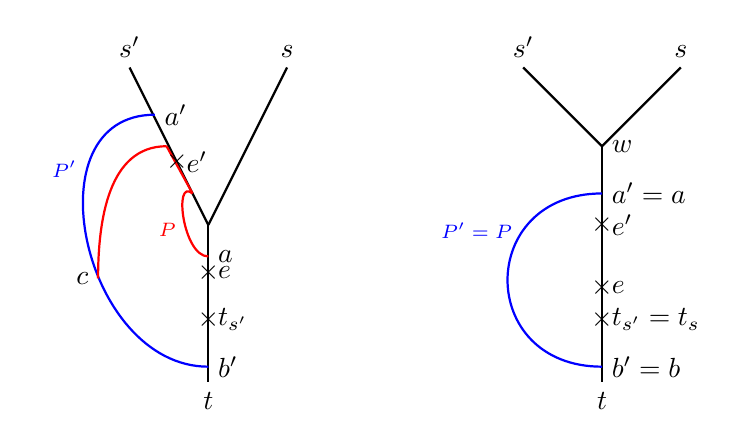
\begin{tikzpicture}[scale=2]
\begin{scope}
\coordinate (s) at (-0.5,2);
\coordinate (s1) at (0.5,2);
\coordinate (w) at (0,1);
\coordinate (t) at (0,0);
\coordinate (ts) at (0,0.4);
\coordinate (b1) at (0,0.1);

\coordinate (i1) at (-0.265,1.5);
\coordinate (i2) at (-0.1,1.2);

\coordinate (a1) at (-0.34,1.7);
\coordinate (a) at (0,0.8);
\coordinate (v) at (0,0.7);
\coordinate (v1) at (-0.2,1.4);
\coordinate (c) at (-0.7,0.66);

\draw[thick](s)--(w);
\draw[thick](s1)--(w);
\draw[thick](w)--(t);
\node[above] at (s){$s'$};
\node[above] at (s1){$s$};
\node[below] at (t){$t$};
\node[right] at (a1){$a'$};
\node[right] at (a){$a$};
\node[right] at (b1){$b'$};
\node[left] at (c){$c$};


\draw[blue,thick] (a1) to[out=180,in=180,distance=.8cm]
node[pos=0.3,left]
{\scriptsize  $P'$}  (b1);

\draw[red,thick] (a) to[out=180,in=140]
node[pos=0.4,left]
{\scriptsize  $P$}  (i2);
\draw[red,thick](i1)--(i2);
\draw[red,thick] (i1) to[out=180,in=90](c);

\node at (v1){$\times$};
\node[right] at (v1){$e'$};

\node at (v){$\times$};
\node[right] at (v){$e$};

\node at (ts){$\times$};
\node[right] at (ts){$t_{s'}$};

\end{scope}
\begin{scope}[xshift=2.5cm]
\coordinate (s) at (-0.5,2);
\coordinate (s1) at (0.5,2);
\coordinate (w) at (0,1.5);
\coordinate (t) at (0,0);
\coordinate (ts) at (0,0.4);
\coordinate (b1) at (0,0.1);

\coordinate (i1) at (-0.265,1.5);
\coordinate (i2) at (-0.1,1.2);

\coordinate (a1) at (0,1.2);
\coordinate (a) at (0.29,1.6);
\coordinate (v) at (0,0.6);
\coordinate (v1) at (0,1);
\coordinate (c) at (-0.7,0.66);

\draw[thick](s)--(w);
\draw[thick](s1)--(w);
\draw[thick](w)--(t);
\node[above] at (s){$s'$};
\node[above] at (s1){$s$};
\node[below] at (t){$t$};
\node[right] at (a1){$a'=a$};
\node[right] at (w){$w$};
\node[right] at (b1){$b'=b$};



\draw[blue,thick] (a1) to[out=180,in=180,distance=.8cm]
node[pos=0.3,left]
{\scriptsize  $P'=P$}  (b1);


\node at (v1){$\times$};
\node[right] at (v1){$e'$};

\node at (v){$\times$};
\node[right] at (v){$e$};

\node at (ts){$\times$};
\node[right] at (ts){$t_{s'} = t_s$};

\end{scope}
\end{tikzpicture}
\caption{ffs}
\label{fig:badexample1}

\end{figure}


On the left hand of the inequality, we  have a path from
$a$ to $t$ avoiding $e$ (since we know that $P$ is a good path, so $P'$ and thus $cb' \conc b't$ does not
pass through $e$). So, its length should be $\ge$
length of the preferred path $P \setminus xa$. Thus $|P
\setminus xa| \le 2|ca|  + |at| \le 2\sqrt {n/\sigma}\
+\ |at|$ (since $|\UNQ(P)| = |ac| < \sqrt{n/\sigma}$). Consider the following set of replacement paths  $(< P)_x
:= \{P' \in (< P)\ |\ P' \ \text{avoids
an edge on $xy$ segment}\}$. By Lemma \ref{lem:avoids},
all  replacement paths in $(<P)_x$ pass through $e$ (as
detour of these replacement paths start below $e$) and by
Lemma \ref{lem:avoidreverse}, these replacement paths avoid
edges that are closer to $y$ than $e$.
  Applying Lemma \ref{lem:length}, we get
that  the number of replacement paths $(<P)_x$  is $ \le 2\sqrt{n/\sigma}$. Thus, once we
get a replacement path $P \in \TTW(xy)$ with $|\UNQ(P)| < \sqrt{n /\sigma}$, then there
are at most $2\sqrt{n/\sigma}$ replacement paths in $\TTW(xy)$ remaining to be processed.
Thus, total number of paths $\in \TTW$ with  $|\UNQ(P)| < \sqrt{n/\sigma}$ is
$\sum_{xy \in \text{\SBFS($t$)}} 2\sqrt{n/\sigma} = O(\sqrt{n \sigma})$
(as there are $O(\sigma)$ segments in \SBFS($t$)).\iflong\\\else\vspace{2mm}\fi

\iflong
   \begin{figure}[hpt!]
\centering
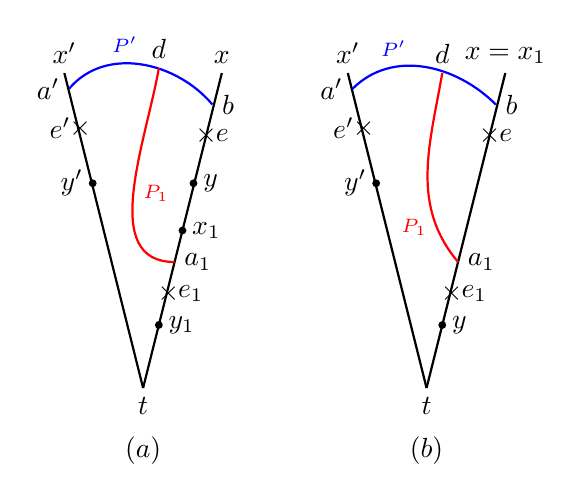
\begin{tikzpicture}[scale=2]
\begin{scope}
\coordinate (s) at (0.5,2);
\coordinate (s1) at (-0.5,2);
%\coordinate (s2) at (1.1,2);
%\coordinate (w) at (0.5,1.4);
\coordinate (t) at (0,0);
\coordinate (ts) at (0.15,0.4);
\coordinate (b) at (0.44,1.8);
\coordinate (y1) at (-0.32,1.3);
\coordinate (y) at (0.32,1.3);

\coordinate (x2) at (0.25,1);
\coordinate (y2) at (0.1,0.4);

\coordinate (a1) at (-0.47,1.9);
\coordinate (a2) at (0.2,0.8);
\coordinate (v) at (0.4,1.6);
\coordinate (v1) at (-0.4,1.65);
\coordinate (v2) at (0.16,0.6);
\coordinate (c) at (-0.7,0.66);
\coordinate (d) at (0.1,2.03);

\draw[thick](s)--(t);
\draw[thick](s1)--(t);
%\draw[thick](s2)--(w);
%\draw[thick](w)--(t);
\node[above] at (s){$x$};
\node[above] at (s1){$x'$};
%\node[above] at (s2){$s_1$};
\node[below] at (t){$t$};
\node[left] at (a1){$a'$};
\node[right] at (b){$b$};

\node[above] at (d){$d$};
%\node[right] at (w){$w$};


\draw[blue,thick] (a1) to[out=50,in=130]
node[pos=0.4,above]
{\scriptsize  $P'$}  (b);



\draw[red,thick] (a2) to[out=180,in=260]
node[pos=0.5,right]
{\scriptsize  $P_1$}  (d);

\node at (v1){$\times$};
\node[left] at (v1){$e'$};


\node[right] at (a2){$a_1$};

\node at (v){$\times$};
\node[right] at (v){$e$};

\node at (v2){$\times$};
\node[right] at (v2){$e_1$};

%\node at (ts){$\times$};
%\node[right] at (ts){$t_{s}$};

\draw (y1) node[fill,circle,scale=0.3]{};
\node[left] at (y1){$y'$};

\draw (y) node[fill,circle,scale=0.3]{};
\node[right] at (y){$y$};

\draw (x2) node[fill,circle,scale=0.3]{};
\node[right] at (x2){$x_1$};

\draw (y2) node[fill,circle,scale=0.3]{};
\node[right] at (y2){$y_1$};

\node at (0,-0.4){$(a)$};

\end{scope}
\begin{scope}[xshift=1.8cm]
\coordinate (s) at (-0.5,2);
\coordinate (s1) at (0.5,2);

\coordinate (t) at (0,0);
\coordinate (ts) at (0.1,0.4);
\coordinate (b) at (0.44,1.8);

\coordinate (a2) at (0.2,0.8);
\coordinate (d) at (0.1,2);
\coordinate (y1) at (-0.32,1.3);
\coordinate (y) at (0.1,0.4);
\coordinate (a1) at (-0.47,1.9);
\coordinate (a) at (0.1,0.8);
\coordinate (v) at (0.4,1.6);
\coordinate (v2) at (0.16,0.6);
\coordinate (v1) at (-0.4,1.65);
\coordinate (c) at (-0.7,0.66);

\draw[thick](s)--(t);
\draw[thick](s1)--(t);

\node[above] at (s){$x'$};
\node[above] at (s1){$x=x_1$};
\node[below] at (t){$t$};
\node[left] at (a1){$a'$};

\node[right] at (b){$b$};
\node[right] at (a2){$a_1$};
\node[above] at (d){$d$};

\draw[blue,thick] (a1) to[out=45,in=135]
node[pos=0.3,above]
{\scriptsize  $P'$}  (b);


\draw[red,thick] (a2) to[out=130,in=260]
node[pos=0.2,left]
{\scriptsize  $P_1$}  (d);

\node at (v1){$\times$};
\node[left] at (v1){$e'$};

\node at (v2){$\times$};
\node[right] at (v2){$e_1$};

\node at (v){$\times$};
\node[right] at (v){$e$};



\draw (y1) node[fill,circle,scale=0.3]{};
\node[left] at (y1){$y'$};

\draw (y) node[fill,circle,scale=0.3]{};
\node[right] at (y){$y$};

\node at (0,-0.4){$(b)$};
\end{scope}
\end{tikzpicture}
\caption{Two cases in which $P'$ passes through $e_1$ after intersecting with $P_1$}
\label{fig:badexample}

\end{figure}

\fi
\noindent  {(2) \em $P$ is a bad path.}
\label{enum:two}

\noindent We now arrive at our hardest scenario.
We will first show that the number of good paths in $\TTW$
is greater than
the number of bad paths in $\TTW$.
To this end, we will prove the following lemma:
\begin{lemma}
\label{lem:badpaths}
For each $P' \in \TTW$, there exists only one replacement
path $P \in \TTW$ which is bad
due to $P'$.
\end{lemma}

\iflong
  \begin{proof}

  Assume that $P$ is the preferred path
  from $x$ to $t$ avoiding $e$ on segment $xy$. Similarly, $P'$ is the preferred path from $x'$ to $t$ avoiding $e'$ on segment $x'y'$ and $P$ is bad due to $P'$. Assume for contradiction that there is one more replacement
  path $P_1$ which is bad
  due to $P'$.
  %, that is,  1)$P_1 \in \TTW \cap (<P')$ and
  %$\DET(P_1)$ intersects with $\DET(P')$ and
  %(2) $\DET(P')$ passes through the edge avoided by $P_1$
  %after their intersection.
  Let us assume that $P_1$ avoids $e_1$ on $x_1y_1$ segment.
  If $x' = x$ or $ x'= x_1$, then $\DET(P')$ cannot pass through
  $e$ or $e_1$ respectively as
  $\DET(P')$ starts before $e$ or $e_{1}$ (as $P' \in (>P)$ or $P' \in (>P_1)$) and touches $x't$ path only at $t_{x'}t$. So, let us assume
  that $x' \neq x$ and $ x' \neq x_1$.

  Since $P' \in \TTW$, by lemma \ref{lem:feature}, we know
  that it follows $xt$ path after hitting segment $xy$, say at $b$. This
  implies
  that $e_1$ also lies on the $xt$ path. Thus, $xt$ and $x_1t$
  intersect. Without loss of generality, assume that  the segment $x_1y_1$ is
  a subpath of $xt$.
  %, say at $w$.
  %Assume without loss of generality
  %that $v_1$ is closer to $t$ than $v$ on $st$ path
  %\begin{enumerate}
  %   \item   $s_1 = s$
  %Note that if $x=x_1$, then $w := x=sx_1$.
  %Without loss of generality assume that $e_1$ is closer to
  %$t$ than $e$. %or $e_1=e$.
  %We have assumed that $P'$ passes through $e$.
  %By Lemma \ref{lem:feature},
  %we know that since $P' \in \TTW$, once it  hits $st$ path
  %(say at $b)$,
  %it cannot leave it.
  %By Lemma \ref{lem:avoids}, $\DET(P_1)$ starts below $v$
  %on $st$ path.
  Let us assume that $\DET(P_1)$ starts at $a_1$ and it
  hits $P'$ at $d$.
  There are two ways for $P_1$ to reach $d$ (both avoiding
  $e_1$):
  $x_1a_1 \conc a_1d$ and $x_1b \conc bd$
  where the first path is using the detour of $P_1$ and the second path
  uses $xt$ path to reach $b$.

  Note that the second path leaves the $x_1t$ path earlier than the
  first path ($x_1$ compared to $a_1$ if $x \neq x_1$ (Figure  \ref{fig:badexample}(a)) and
  $b$ compared to $a_1$ if $x=x_1$ (Figure  \ref{fig:badexample}(a))). Even then the preferred
  path used the first alternative.
  This implies that the length of the first path
  must be {\em strictly} less than the second.  Thus,
  $|x_1a_1| + |a_1d| < |x_1b| + |bd|$. Thus,
  \begin{equation}
  |a_1d| < |db| + |bx_1| - |x_1a_1|
  \end{equation}
  $P'$ takes the following path
  $x'a' \conc a'b \conc bt$.
  But there is  an alternative path available for $P'$, it
  is $x'a' \conc a'd \conc da_1 \conc a_1t$.
  The path is a valid path avoiding $e'$ only if $a_1d$
  does not pass through $e'$. All other components of this
  path are a part of $P'$ ($a'd \in a'b$ and $a_1t \in bt$)
  .

  If $a_1d$ does not pass through $e'$, then we can show that
  the alternative path has a length less than $|P'|$, thus arriving
  at a contradiction.
  Consider the length of the alternative path:
  \begin{tabbing}
   $|x'a'| $\=$+ |a'd| + |da_1| + |a_1t|$\\
   \>$< |x'a'|+ |a'd| + |db|  + |bx_1| - |x_1a_1| + |a_1t|$
  \hspace{10mm}\ (Using  Equation (1))\\\\
  If $x \neq x'$(See Figure  \ref{fig:badexample}(a)), then
  $ |bx_1|  - |x_1a_1|
  + |a_1t| \le  |bx_1|  + |x_1a_1| + |a_1t| = |bt|$. Else if $x
  =x'$ \\
  (See Figure  \ref{fig:badexample}(b)), then $ |bx_1|  - |x_1a_1|
  + |a_1t| = -|ba_1| +\ |a_1t| \le|ba_1| +\ |a_1t| =  |bt|$ \\\\
   \>$\le |x'a'|+ |a'd| + |db| + |bt|$\\
  \>$= |x'a'|+ |a'b| + |bt|$\\
   \>$= |P'|$
  \end{tabbing}

  This leads to a contradiction as we have assumed that $P'$
  is
  the shortest path from $x'$ to $t$ avoiding $e'$.

  To end this proof, we will show that $a_1d$ cannot pass
  through $e'$.
  Assume for contradiction that $a_1d$ passes through $e'$.
  This
  implies that $\DET(P_1)$ intersects with $x'y'$ segment (as
  $e' \in x'y'$) and
  then diverges from it (as $\DET(P_1)$ intersect with $\DET(P')$
  at $d$).
  By Lemma \ref{lem:feature}, $P_1 \notin \TTW$. But this cannot
  be the
  case as we have assumed that $P_1 \in  \TTW$. Thus our assumption,
  namely $a_1d$ passes through $e'$ must be false.


  %\item $s''=s$

  %Assume without loss of generality \todo{Is this wlog fine}
  %that $e''$ lies below $e$ on $st$ path. By Lemma \ref{},
  %we know that $P'$ leaves $st$ above $e$ and merges back
  %only at $t_st$ path. Since $e' \notin t_st$, this implies
  %that $P'$ can never pass through $e'$. Thus, we arrive
  %at a contradiction.

  %\item $s_1 \neq s$

  %Since $P' \in \TTW$, by lemma \ref{lem:feature}, we know
  %that it follows $st$ path after hitting it. This implies
  %that $v_1$ also lies on the $st$ path. Thus, $st$ and $s_1t$
  %intersect, say at $w$. Assume without loss of generality
  %that $v_1$ is closer to $t$ than $v$ on $st$ path. So,
  %$P_1$ satisfies two condition: (1) It intersects with $P'$
  %and (2) The vertex avoided by $P'$ is closer to $s$ than
  %$v''$. By Lemma \ref{}, we infer than $P'' \in \TON$. Thus,
  %we again arrive at a contradiction.

  %\end{enumerate}
  \end{proof}
\fi




%We now put the above lemma to use. We use the following
%algorithm to weed out paths that satisfy case 1(b) and case
%2.

%\begin{algorithm}
%\ForEach{$P \in \TTW$ precessed according to the ordering
%$\prec$}
%{
%    $\BP \leftarrow \emptyset$; \tcp{Set of Bad Paths}

%    $\GP \leftarrow \emptyset$; \tcp{Set of Good Paths}

%    \If{$\exists$ \ \text{a path in $GP$ whose detour start
%at the same vertex as of $P$\ }}
%    {
%        continue;
%    }
%    \If{ $\exists P' \in \GP$ such that $P'$ passes through
%$e$ after intersecting $P$ }
%    {

%        $\BP \leftarrow \BP \cup  \{P\}$\;
    % }
%     \Else
%     {
%         $\GP \leftarrow \GP \cup \{P\}$\;
%     }
% }
% \end{algorithm}

% The above algorithm discards a path $P$ if there already
% exists a processed good path whose detour starts from the
% same vertex as that of $P$. This takes care of case \ref{enum:one}.
% It then removes all the replacement paths $P$ that satisfy
% the conditions in Case \ref{enum:two}. $\BP$ is the set
% of paths removed by the algorithm. For each such path, there
% exists a path $P' \in \GP$. By Lemma \ref{lem:badpaths},
% we know that each good path in $\GP$ can remove atmost one
% bad path. This implies that the number of bad paths removed
% is $\le$ number of good paths, that is $|\BP| \le |\GP|$.
% All the paths in $\GP$ do not satisfy case \ref{enum:one}
% and \ref{enum:two}. Thus, these paths satisfy  case \ref{enum:goodcase}.

The above lemma can be used to discard bad paths from $\TTW$.
For each such discarded path, there exists at least one good path.
And by the above lemma, each such good path can be used to discard
at most one bad path. Thus the number of good paths in $\TTW$
is $\ge$ number of bad paths in $\TTW$.
We have already shown that the total number of good paths in $\TTW$
is $O(\sqrt{n\sigma})$.
Thus the total number of paths in $\TTW$ is also $O(\sqrt{n\sigma})$.

% Let $wy$ be a segment in \SBFS($t$) where $y$ is closer
% to $t$ than $w$.
% Let $\TTW(w)$ denote the set of all replacement paths in
% $\TTW$ whose detour
% start in segment $wx$. $\TTW(w)$ can be implemented as a
% balanced binary
% search tree.
%  Since size of $\TTW$ is $O(\sqrt{n \sigma})$, the size of $\cup_{w \in \text{\SBFS($t)$}}\ |\TTW(w)| = O(\sqrt{n \sigma})$.

% !TEX root = paper.tex
\iflong
\else
\vspace{-2mm}
\fi
\iflong
\else
\begin{figure}[hpt!]
\centering

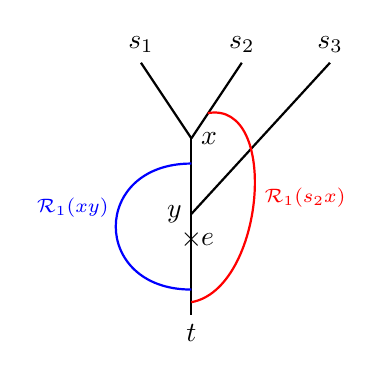
\begin{tikzpicture}[scale=1.6]
\begin{scope}
\coordinate (s2) at (0.4,2);
\coordinate (s1) at (-0.4,2);
\coordinate (s3) at (1.1,2);
\coordinate (x) at (0,1.4);
\coordinate (y) at (0,0.8);
\coordinate (t) at (0,0);
\coordinate (ts) at (0.15,0.4);
\coordinate (b1) at (0,.2);


\coordinate (a1) at (0,1.2);
\coordinate (a2) at (0.13,1.6);
\coordinate (v) at (0,.6);

\coordinate (c) at (-0.7,0.66);
\coordinate (b2) at (0,0.1);

\draw[thick](s1)--(x);
\draw[thick](s3)--(y);
\draw[thick](s2)--(x);
\draw[thick](x)--(t);
\node[above] at (s2){$s_2$};
\node[above] at (s1){$s_1$};
\node[above] at (s3){$s_3$};
\node[below] at (t){$t$};


\node[left] at (y){$y$};
\node[right] at (x){$x$};


\draw[blue,thick] (a1) to[out=180,in=180,distance=.8cm]
node[pos=0.4,left]
{\scriptsize  $\TON(xy)$}  (b1);



\draw[red,thick] (a2) to[out=10,in=10]
node[pos=0.5,right]
{\scriptsize  $\TON(s_2x)$}  (b2);

\node at (v){$\times$};
\node[right] at (v){$e$};

\end{scope}

\end{tikzpicture}
\caption{The shortest path from $s_2$ to $t$ avoiding $e$ can be $\TON(xy)$ or $\TON(s_2x)$.}
\label{fig:heavylight}

\end{figure}

\fi
\section{Building the Data Structure}
\iflong
\else
\vspace{-4mm}
\fi
\label{sec:data}

Let us first recognize a potential problem in using $\TON(\cdot)$.
%Consider a segment $xy$. We know that $\TON(xy)$ is a replacement path from $x$ to $t$ avoiding $yt_x$. We store only one path from $\TON$ for the segment $xy$   as
%we don't have enough space to store all the paths. However, this strategy leads to the following
%problem.
Let $s_1t$ and $s_2t$ path  meet at vertex $x$ (See Figure \ref{fig:heavylight}).
Another path $s_3t$
 meets $s_2t$ path at $y$ where $y$ is closer to $t$.
$\TON(s_2x)$ is the shortest path from $s_1$ to $t$ avoiding $e$ and $\TON(xy)$ is the shortest path from
$x$ to $t$ avoiding $e \in yt $. This immediately leads to the following problem. Assume that
the query is $\textsc{Q}(s_2,t,e)$ and the preferred path avoiding $e$ is in $\TON$.
Then there are two  candidate paths that avoid
$e$: one that goes from $s_2$ to the intersection vertex $x$ and then take
path  $\TON(xy)$ and the other $\TON(s_2x)$.
Thus, we need to check these two paths and return the minimum of the two. One can
make a bigger example in which there are $\sigma$ segments between $s_2$ and $t$
and thus we have to check $O(\sigma)$ path before we can answer the query. The problem appears
because we don't know from which segment the shortest path avoiding $e$ started its detour.
If this information is not there, then it seems that we have to look at all the segments between
$s_2$ ans $t$.
\iflong
\begin{figure}[hpt!]
\centering

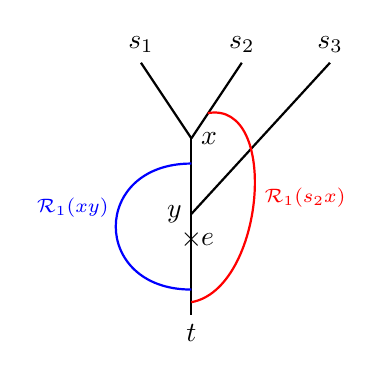
\begin{tikzpicture}[scale=1.6]
\begin{scope}
\coordinate (s2) at (0.4,2);
\coordinate (s1) at (-0.4,2);
\coordinate (s3) at (1.1,2);
\coordinate (x) at (0,1.4);
\coordinate (y) at (0,0.8);
\coordinate (t) at (0,0);
\coordinate (ts) at (0.15,0.4);
\coordinate (b1) at (0,.2);


\coordinate (a1) at (0,1.2);
\coordinate (a2) at (0.13,1.6);
\coordinate (v) at (0,.6);

\coordinate (c) at (-0.7,0.66);
\coordinate (b2) at (0,0.1);

\draw[thick](s1)--(x);
\draw[thick](s3)--(y);
\draw[thick](s2)--(x);
\draw[thick](x)--(t);
\node[above] at (s2){$s_2$};
\node[above] at (s1){$s_1$};
\node[above] at (s3){$s_3$};
\node[below] at (t){$t$};


\node[left] at (y){$y$};
\node[right] at (x){$x$};


\draw[blue,thick] (a1) to[out=180,in=180,distance=.8cm]
node[pos=0.4,left]
{\scriptsize  $\TON(xy)$}  (b1);



\draw[red,thick] (a2) to[out=10,in=10]
node[pos=0.5,right]
{\scriptsize  $\TON(s_2x)$}  (b2);

\node at (v){$\times$};
\node[right] at (v){$e$};

\end{scope}

\end{tikzpicture}
\caption{The shortest path from $s_2$ to $t$ avoiding $e$ can be $\TON(xy)$ or $\TON(s_2x)$.}
\label{fig:heavylight}

\end{figure}

\fi
To end this dilemma, we use heavy light decomposition of \SBFS($t$) \cite{SleatorT83}.
For any segment $xy \in$ \SBFS($t$) (by our convention $y$ is closer to $t$), $x$ is a {\em heavy}
child of $y$ if the number of nodes in the subtree under $x$ is $\ge$ 1/2(number of
nodes in the subtree under $y$) else it is called a {\em light child} (or light {\em segment} in our case).
%$x$ is also called the {\em heavy child} of $y$.
It follows
that each intersection vertex has exactly one heavy child and
each vertex is adjacent to atmost two heavy edges. A {\em heavy chain} is a concatenation of
heavy edges. A {\em heavy subpath} is a subpath of a heavy chain.
The following lemma notes a well known property of heavy-light decomposition.

\begin{lemma}
\label{lem:decomposition}
The path from a source $s$ to $t$ in \SBFS($t$) can be decomposed into $O(\log n)$ heavy subpaths
and light segments .
\end{lemma}

Given any source $s \in S$, by Lemma \ref{lem:decomposition},
the path from $t$ to $s$
may contain many heavy subpaths.
Let $C(pq)$ be a heavy
chain that starts at $p$
and ends at $q$ (where $q$ is closer to $t$ than $p$). A $ts$ path may follow
a heavy chain $C(pq)$ but may exit
this chain from a vertex midway, say at $r$. Let $(C(pq), r)$
be a tuple associated with $s$
such that the shortest path from $t$ to $s$ enters this
heavy chain via $q$ and
leaves this chain at $r$. We keep a list $\HE(s,t)$
which contains
all the tuples $(C(pq), r)$ sorted according to
the distance of heavy chain
from $t$ (that is distance $qt$). By Lemma \ref{lem:decomposition},
the size
of $\HE(s,t) = O(\log n)$. Similarly, we have one more
list to store the light segments.
$\LI(s,t)$ contains all the light segments on the $st$ path
again ordered according to their
distance from $t$ in \SBFS($t$). Again by Lemma  \ref{lem:decomposition},
the size
of $\LI(s,t) = O(\log n)$. Note that the size of these additional
two data-structures
is $\sum_{s \in S} O(\log n) = \tilde O(\sigma) = \tilde O(\sqrt{n\sigma})$.


Our main problem was that we have to find the minimum $\TON(\cdot)$ of $O(\sigma)$ segments if 
there is a path of length $\sigma$ between $s$ and $t$. The trick we use here is that
finding minimum on any heavy subpath takes $\tilde O(1)$ time. Since
there are $O(\log n)$ heavy subpaths, the total time taken to find the minimum
on heavy subpaths in $\tilde O(1)$. Also, since the number of light segments is also $O(\log n)$
finding the minimum among these also takes $\tilde O(1)$ time.

We now describe our intuition in detail.  Let $xy$ be a segment in a heavy chain
$C(pq)$. We want to represent $\TON(xy)$ in a
balanced binary search tree $\BST(C)$. To this end, we will add a node with
the tuple $(x.depth,| px \conc \TON(xy) |, |px|)$  in $\BST(C)$.
The first element in this tuple is the depth of $x$
in $\BFS(t)$ --  it also acts as the key in this binary search tree. The second element
is the path $ \TON(xy)$  concatenated with $px$. This concatenation is done so that all  paths
in $\BST(C)$ start from $p$ and comparing two paths in $\BST(C)$ is
possible. The third element will be used to get the path length $\TON(xy)$ (by subtracting it from
the second element) when
need arises. Now we can augment
this tree so that the following range minimum query can be answered in $\tilde O(1)$ time:
$\RMQ(C(pq),[a,b])$ : Find minimum of $\{|px \conc \TON(xy)|\ |\ xy \ \text{is a segment in heavy chain $C(pq)$ and }\ x.depth \ge a.depth \ \text{and}\  x.depth \le b.depth \}$.
The size of $\cup_{C \in \HE(s,t)}\BST(C)$ is $O(\sigma) = O(\sqrt{n\sigma})$ as there are
at most $O(\sigma)$ segments in \SBFS($t$).
\iflong
\begin{algorithm}
\SetKwRepeat{Do}{do}{while}%
  \caption{Finding the shortest replacement path  (in $\TON$) from $s$ to $t$ avoiding $e(u,v)$ }
  \label{fig:findR1R2}
Let $x$ be  the first intersection point on $us$ path\;
$min \leftarrow \infty$ \;

\Do{$x$ is not equal to $s$ }
{
    \If{ $x$ lies in a heavy chain}
    {
        Using $\HE(s,t)$, find $(C(pq),r)$, that is $r$ is the vertex from which $us$
        path leaves the chain $C$\;
        $min\leftarrow \min\{ min, \RMQ(C, [x,r]) - |pr| + |sr| \}$\;
        $x \leftarrow r$\;
    }
    \ElseIf{$x$ is an endpoint of a light segment}
    {
        Let $x'x$ be the  light segment ending at $x$ in \SBFS($t$) \tcp*{Can be found out via $\LI(s,t)$ in $\tilde O(1)$ time.}

        $min \leftarrow \min\{ min, |\TON(x'x)| + |sx'| \}$\;
        $x \leftarrow x'$\;
    }
}
\end{algorithm}
\fi


Given any edge $e(u,v)$ on $st$ path, we can now find the shortest path in $\TON$ from
$s$ to $t$ avoiding $e$
\iflong
(see Algorithm \ref{fig:findR1R2}).
\else
(Please refer to Algorithm \iflong\ref{fig:findR1R2}\else 1\fi~ in the full version of the paper).
\fi We first find the first intersection vertex on the
$us$ path from $u$. Let this vertex be $x$. We will see that finding
$x$ is also not a trivial problem --  we will say more about this problem later.
Now, we will go over all  possible replacement paths from $u$ to $s$.
Thus, we  search if there exists any heavy chain in
$\HE(s,t)$ that contains $x$. To this end, we first check if $x$ lies in some light segment (this can be checked in $\tilde O(1)$ time). If not, then $x$ lies in some heavy chain. We now search each heavy chain in $\HE(s,t)$ to find a node $x'$ with the smallest depth such that  $x'.depth > x.depth$.
Let this node be $x'$. Thus we have found the segment $x'x$ where $x$ is closer to $t$
than $x'$.
%where $x.depth$ is the depth of $v$ in $\BFS(t)$.
We can easily calculate $x.depth$ as
$|st| - |sx|$ or $B_0(s,t) - B_0(s,x)$. Since there are $\tilde O(1)$ heavy
chain in $\HE(s,t)$, the time taken to find if $x'x$ exists in some heavy chain is $\tilde O(1)$.
%Similarly, the reader can infer that the time taken to %find the light segment
%in which $x$ is an endpoint is $\tilde O(1)$.
%Once we have found such a
%heavy path or light segment, then we check if the replacement %lies on it.

Assume that we found out that
$x'x \in C(pq)$,  and $ts$ path leaves the chain $C$ at $r$, then we want to
find the shortest replacement path from $r$ to $t$ avoiding $e$. This can be found out via the range minimum query $\RMQ(C(p,q),[x,r])$.
However, note that each replacement path in $C$ starts from $p$. So, we need to
remove $|pr|$ from the replacement path length returned by $\RMQ$ query.
The length $pr$ can be found out in the node $r \in \BST(C)$. Finally, we add $|sr|$ to get the path from $s$ to $t$.

Similarly, we can process a light segment in $O(1)$ time (please refer to Algorithm \iflong\ref{fig:findR1R2}\else
1 in the full version\fi~).
Thus, the time taken by  Algorithm  \iflong\ref{fig:findR1R2}\else
1\fi~ is
$\tilde O(1)$ as the while loop runs at most $O(\log n)$ times  and each step in
the while loop runs in $\tilde O(1)$ time.



%The above algorithm moves from vertex $u$ to $s$, that is $us$ path.
%If it encounters a light edge $vv'$ in this path then it, then we check if the
%$st$ path whose detour starts on $vv'$ is the minimum, that is path $sv' \conc \TON(v')$.
%Else, if we encounter a heavy chain, then we

\begin{comment}
We are now ready to describe our data-structure to process queries. We first need
to check the vertex to be avoided is an intersection point in \SBFS$(t)$. To this end,
we check if the vertex exists in $\BST_1(t)$. If yes, then we return the length of the
preferred path associated with the vertex. The size of
$\BST_1(t)$ is $O(\sigma) = O(\sqrt{n \sigma})$ as there are $O(\sigma)$ intersection
point in \SBFS$(t)$.


Let $xy$ be a segment in \SBFS$(t)$.  We will associate two data structures with
$x$, (1) $D_0(x,t)$ contains   the preferred replacement path from $x$ to $t$
such that its detour starts in segment $xy$, but the avoided vertex lies in $yt$,
that is, that path in $\TON$ (2) $\BST_2(x,t)$ contains all the  preferred path
from $x$ to $t$ such that their detour start in segment $xy$ and the avoided
vertex also lies in $xy$, that is, paths in $\TTW$. As in the single source case,
we first show that each path in $\BST_2(x,t)$ avoid a contiguous subpath of $xy$.

By Corollary \ref{cor:arrange}, we can arrange paths in $\BST_2(x,t)$ in decreasing order of their length. By
Lemma \ref{lem:avoids}, for any two path $P,P' \in \BST_2(x,t)$, if $|P| > |P'|$, then $\DET(P')$
starts below the vertex avoided by $P$. This lemma implies
that $\DET(P')$ starts below all the vertices avoided by
$P$. Thus $P$ avoids some contiguous path in $xy$ path.
We can $\BST_2(x,t)$ as a balanced binary search tree. For each subpath $zz'$ of $xy$,
we store the length of the replacement path from $x$ whose detour starts before $z$ and it
meets $xt$ path again in $t_xt$.  Additionally, we also store the distance of $z$ and $z'$
from $x$. These distances will act as the key of a node in $\BST_2(x,t)$.
\end{comment}
\iflong
\else
\vspace{-2mm}
\fi
\subsection{Answering queries in $\tilde O(1)$ time}
\iflong
\else
\vspace{-2mm}
\fi
Given a query ${\sc Q}(s,t,e(u,v))$, we process it as follows
(assuming that $e$ lies on $st_s$ path (that is the {\em far case)} and $v$ is closer to $t$ than $u$)\iflong\\\else\vspace{1mm}\fi


\begin{comment}
{\em (1) Check if $e$ lies on $st_s$ path.}

  Since all the shortest path have unique length, we find if $|su|_{p} + |ut_s| _{p}+ |t_st|_{p} = |st|_p$. To this end, we use the data structure already defined in Section \ref{}. We first find $t_s \leftarrow
  B_2(s,t)$.
  Then we check if $B_0^{p}(s,u) +\ B_0^{p}(u,t_s) +\ B_0^{p}(t_s,t)
  = B_0^{p}(s,t)$.

  \item Check if $u$ is an intersection vertex in \SBFS$(t)$.

  For each $t$ we build a balanced binary search tree that stores all the intersection vertex in $\BFS(t)$. Since the number of intersection vertex in $\BFS(t)$ is $O(\sigma)$, the size of this binary search tree is $O(\sigma) = O(\sqrt{n \sigma})$. We then check now check  $u$ is an intersection vertex in  $\tilde O(1)$ time.

\end{comment}

\begin{enumerate}[leftmargin=*,noitemsep,nolistsep]
\item Find the first intersection vertex  on $us$ path.

\iflong
  \noindent As we have mentioned before, this is not a trivial problem.
  Let the first intersection vertex from $u$ to $s$ in $\BST(t)$ be
  denoted by  $\INT_{s}(u,t)$.   We will first show that $\INT_{s}(u,t)$ is independent of $s$.
  \begin{lemma}
  \label{lem:intlemma}
  $\INT_s(u,t) = \INT_{s'}(u,t)$ for $s,s' \in S$ for all $u \in \BFS(t)$.
  \end{lemma}

  \iflong
  \begin{proof}
    We will prove this by induction on the nodes of $\BFS(t)$ from leaf to root $t$.
    The base case is a leaf in $\BFS(t)$, that is a source vertex, which by definition,
    itself is an intersection vertex. For any node $u$, if $u$ is an intersection vertex,
    $\INT_s(u,t) = \INT_{s'}(u,t) = u$. Else, $u$ is a node of degree 2 in $\BFS(t)$.
    Assume that $u'$ is the child of $u$ in $\BFS(t)$. So, $\INT_s(u,t) = \INT_s(u',t)$ and $\INT_{s'}(u,t) = \INT_{s'}(u',t)$. But by induction hypothesis,  $\INT_s(u',t)=\INT_{s'}(u',t)$.

    \end{proof}
  \fi

  \noindent We will drop the subscript $s$ from the definition of $\INT(\cdot,\cdot)$ as we now know that it is independent of $s$. We use the
  above lemma to construct  two data structures that will help us in finding $\INT(u,t)$.

  \begin{itemize}
  \item $I_1(t)$: For any $u \in V$, if $\INT(u,t)$ is within a distance of $c\sqrt{n/\sigma} \log n$
  (for some constant $c$) from $u$, then we store the tuple
  $(u,\INT(u,t)$) in the balanced binary search tree $I_1(t)$. For any  intersection
  vertex $x \in $ \SBFS$(t)$, we  store at most $\tilde O(\sqrt{n/\sigma})$ tuples in $I_1(t)$.
  For a fixed $t$, the total
  space taken by $I_1(t)$ is $\tilde O(\sigma .\sqrt{(n/\sigma)}
  )= \tilde O(\sqrt{n \sigma})$ (as there are $O(\sigma)$ intersection vertices in \SBFS($t)$.
  %Given a vertex $u$, we then try to find if $u$
  %exists in this data-structure. This takes $\tilde O(1)$
  %time.

  \item $I_2(t)$: If $u$ is not present in $I_1(t)$, then $\INT(u,t)$ is at a distance
  $\ge c\sqrt{n /\sigma}\log n$ from $u$. We now
  use a different strategy to find $\INT(u,t)$. We first find $u_s \leftarrow B_1(s,u)$,
  that is the vertex in $\TT$
  closest to  $u$ in $su$ path. With a
high probability,
$u_s$ is closer to $u$ than $\INT(u,t)$ and all the vertices from $u$ to $u_s$ have degree  exactly 2 in $\BFS(t)$.
  Thus, $\INT(u_s,t) = \INT(u,t)$ -- we will now use this property (a similar property was also used in the proof of Lemma \ref{lem:intlemma}).

  \begin{comment}
        \begin{figure}[hpt!]
        \begin{algorithm}[H]
        \If{$u \in I_1(t)$}
        {
            return $I_1(u,t)$;
        }
        \Else
        {
            $u_s \leftarrow B_1(s,u)$\;
            return $I_2(u_s,t)$;
        }
        \end{algorithm}
        \caption{\textsc{Find-Int}$(s,u,t)$: An algorithm to find $\INT_s(u,t)$}
        \end{figure}
  \end{comment}
  \noindent
  For each $x \in \TT$
  such that $x$ is not an intersection vertex in $\BFS(t)$, we store the tuple
  $(x,\INT(x,t))$ in another balanced binary search tree $I_2(t)$. For a fixed vertex $t$, the
  size of this data-structure is $\tilde O(\sqrt{n\sigma})$ space
  as there is only one intersection vertex for each vertex
  in $\TT$ and $|\TT| = \tilde O(\sqrt{n \sigma})$

\end{itemize}
  \noindent If $\INT(u,t)$ is indeed at a distance $\le
c \sqrt{n / \sigma} \log n$,
  then we can use $I_1(t)$  to find it in $\tilde O(1)$
time, else we use $I_2(t)$ to find
  $\INT(u_s,t)$ in $\tilde O(1)$ time.\\

  \begin{comment}
  \noindent {\em Assuming $x = \INT_s(u,t)$,  find $\INT_s(x,t)$}

  Our aim is to find the segment which ends at $x$ in \SBFS($t)$. To this end,
  we find $\INT(x,t)$. To this end, we use another balanced binary search tree.
  For each intersection vertex $v \in $ \SBFS($t$), we store the tuple
  $(s,\INT_s(v,t))$ in $I_3(v,t)$. Unlike non intersection vertex, for an
  intersection vertex $v$, $\INT_s(v,t)$ may be dependent on $s$.

  \end{comment}
\else
\noindent In the full version of the paper, we show that we can find the first intersection vertex  on $us$ path
in $\tilde O(1)$ time using $O(\sqrt{n\sigma} )$ space.
\fi
\item Find  the replacement path avoiding $u$  if it lies in $\TON$.
\label{fcase1}

\noindent To this end, we use our Algorithm \iflong\ref{fig:findR1R2}\else
1\fi.
The first non-trivial part of this algorithm, that is, finding the first
intersection vertex on the $us$ path has already been tackled in the point above.
So we can find such a replacement path (if it exists) in
$\tilde O(1)$ time  and $\tilde O(\sqrt{n \sigma})$ space.\iflong\\\else\vspace{1mm}\fi


\item Find the replacement path avoiding $e(u,v)$ if it lies in $\TTW$.
\label{fcase2}

\noindent  This part is similar to our data-structure in single source case.
Let $x \leftarrow \INT(u,t)$.  Using $\HE(s,t)$ and $\LI(s,t)$, in $\tilde O(1)$ time,
we can find the segment $xy \in $ \SBFS($t$) such that $y$ is closer to $t$ than $x$.
In this case, we want to check if there exists any
replacement path that starts in  the  same segment in which
$e$ resides. This  replacement path first takes $sx$ path and then takes
 the  detour strictly inside  the  segment $xy$. All such paths are stored in $\TTW(xy)$
with the contiguous range of edges that they avoid on $xy$.
We now just need to check if $u$ and $v$ lie in the range of some replacement path.
To this end, we find $u.depth \leftarrow |st| -|su| = B_0(s,t) - B_0(s,u)$
and $v.depth \leftarrow |st| -|sv| = B_0(s,t) - B_0(s,v)$.
Now we check if $u.depth$ and $v.depth$ lie in contiguous range of
some replacement path  in $\TTW(xy)$. If yes, then we return the length of that
path concatenated with $sx$.  Note that we have already stored $|sx|$ in $B_0(s,x)$.
The time taken in this case is dominated by searching $u$ and $v$ in $\TTW(xy)$,
that is $\tilde O(1)$.\iflong\\\else\vspace{1mm}\fi
\end{enumerate}

\noindent Thus, the total query time of our algorithm is $\tilde O(1)$, and we can return the
minimum of replacement paths found in Step \ref{fcase1} and \ref{fcase2} as our final answer.
The reader can check that the space taken by our algorithm for a
vertex $t$ is $\tilde O(\sqrt{n\sigma})$. Thus the total space taken by our algorithm is
$\tilde O( \sigma^{1/2} n^{3/2}) $. Thus we have proved the main result, that is Theorem \ref{thm:maintheorem} of our paper.

%\begin{theorem}
%There exists a data-structure of size $\tilde O(\sigma^{1/2}n^{3/2})$
%for multiple source single fault tolerant exact distance oracle
%that can answer each query in $\tilde O(1)$ time.
%\end{theorem}


\bibliographystyle{plain}
\bibliography{sample}

\end{document}
